%% Semplice beamer conforme al powerpoint ufficiale
%% dal sito di Ca' Foscari. Si basa sul tema "default"
%% mandate Modifiche e migliorie! Guido.Caldarelli@unive.it 
% Elenco Contributori 
% Guido Caldarelli, Matteo Brilli 

%\documentclass{beamer}
% decide below the aspect ratio between 16:9 and 4:3
%\documentclass[aspectratio=43]{beamer}
\documentclass[aspectratio=169, 11pt]{beamer}

\usepackage[utf8]{inputenc}
\usepackage{tikz}
\usepackage{multicol}
\usetikzlibrary{tikzmark, shapes}
\usepackage{bm}
\usepackage[dvipsnames]{xcolor}
\usepackage{graphicx}  % Required for \settowidth
% Questo tema commentato di sotto produce un beamer più tradizionale 
%\usetheme[secheader]{Boadilla}


%%%-----------------------------------------------------------%
%% Cambia colori da thema default
%% Questi sono i due colori ufficiali rosso e grigio
\definecolor {cfred}{rgb}{0.709,0.196,0.329} 	%{ 181 ,50 ,84}
\definecolor {cfgrey}{rgb}{0.537,0.537,0.537} 	%{ 137,137,137}
\definecolor {cflink}{rgb}{0.615,0.615,0.607} 	%{157,157,155}
\definecolor {cfgreen}{rgb}{0.004, 0.196, 0.125} %{1, 50, 32}

\setbeamercolor{palette primary}{bg=cfred,fg=white}
\setbeamercolor{palette secondary}{bg=cfred,fg=white}
\setbeamercolor{palette tertiary}{bg=cfred,fg=white}
\setbeamercolor{palette quaternary}{bg=cfred,fg=white}
\setbeamercolor{palette five}{bg=cfgreen, fg=white}
\setbeamercolor{structure}{fg=cfred}		 % itemize, enumerate, etc
\setbeamercolor{section in toc}{fg=cfred} 		 % TOC sections
% Override palette coloring with secondary
\setbeamercolor{subsection in head/foot}{bg=cfgrey,fg=white}
%%%------------------------------------------------------------

%% Definisce il blocco con riquadro che non è presente nel tema default (commentare se si usano altri temi)
\setbeamercolor{uppercolor}{fg=white,bg=cfred}%
\setbeamercolor{lowercolor}{fg=black,bg=white}%
\def \bblock{\begin{beamerboxesrounded}[upper=uppercolor,lower=lowercolor,shadow=true]}
\def \eblock{\end{beamerboxesrounded}}
%%-----------------------------------------------------------
%\setbeamertemplate{footline}[frame number]
% Customize the footline
\setbeamertemplate{footline}{%
  \leavevmode%
  \hbox to \paperwidth{%
    % First box (Email address) - Exactly 1/3 of paperwidth
    \begingroup
    \setlength{\fboxsep}{2pt}% Padding inside the box
    \colorbox{cfred}{\makebox[\dimexpr0.333\paperwidth\relax][c]{\strut\textcolor{white}{\texttt{myp23@cam.ac.uk}}}}%
    \endgroup
    % Second box (Custom text) - Exactly 1/3 of paperwidth
    \begingroup
    \setlength{\fboxsep}{2pt}% Padding inside the box
    \colorbox{cfred}{\makebox[\dimexpr0.333\paperwidth\relax][c]{\strut\textcolor{white}{2411.17663}}}%
    \endgroup
    % Third box (Frame number) - Exactly 1/3 of paperwidth
    \begingroup
    \setlength{\fboxsep}{2pt}% Padding inside the box
    \colorbox{cfred}{\makebox[\dimexpr0.334\paperwidth\relax][c]{\strut\textcolor{white}{\insertframenumber/\inserttotalframenumber}}}%
    \endgroup
  }%
  \vskip0pt%
}
\setbeamertemplate{caption}{\raggedright\insertcaption\par}
%% Intestazione ripetuta per ogni slide
\addtobeamertemplate{headline}{%
\vspace{0.25cm} \ \ 

\includegraphics[height=1.0cm]{Ca_Foscari Beamer/cambridge-cropped.pdf}

\includegraphics[height=1.0cm]{kicc.png} 	% sostituire con logobeamIT.png per italiano
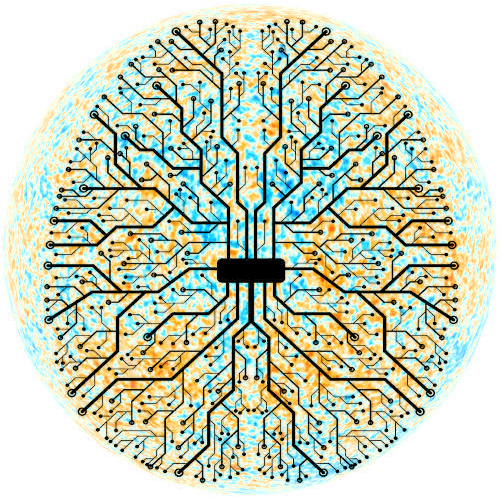
\includegraphics[height=1.0cm]{Ca_Foscari Beamer/handley-lab.png}
%\hspace{0.641\textwidth}{\color{cflink} {\small www.unive.it}} %per 16:9
%\hspace{0.551\textwidth}{\color{cflink} {\small www.unive.it}} %per 4::3
\vspace{0.25cm}
{\color{cfred} \hrule \hrule  }
\textbf{}
}{}
%%-------------------------------------------------------------

%This block of code defines the information to appear in the Title page
%%%
\title[Accelerated nested sampling with $\beta$-flows for gravitational waves] %optional
{Accelerated nested sampling with $\beta$-flows}

\author[Metha Prathaban] % (optional)
{Metha Prathaban \break myp23@cam.ac.uk \break \vfill
\includegraphics[width=0.22\textwidth]{Ca_Foscari Beamer/qr-code.png}}
\date{}



\setbeamertemplate{frametitle}[default][right, rightskip=.5cm] {}
\addtobeamertemplate{frametitle}{\vspace*{-1.4cm}}{}
\setbeamertemplate{navigation symbols}{}
%End of title page configuration block
%------------------------------------------------------------


%------------------------------------------------------------
%The next block of commands puts the table of contents at the 
%beginning of each section and highlights the current section:

\AtBeginSection[]
{
  \begin{frame}
    \frametitle{Table of Contents}
    \tableofcontents[currentsection]
  \end{frame}
}
%------------------------------------------------------------

\begin{document}

%The next statement creates the title page.
\frame{\titlepage}
%---------------------------------------------------------
%This block of code is for the table of contents after
%the title page
\begin{frame}
\frametitle{About Me}
\begin{itemize}
    \item 3rd year PhD student
    \item Work on Bayesian numerical method development in context of GWs
\end{itemize}
\vspace{2em}
\bblock{\begin{center}
Current work is in collaboration with Will Handley and Harry Bevins.
\end{center}}
\begin{center}
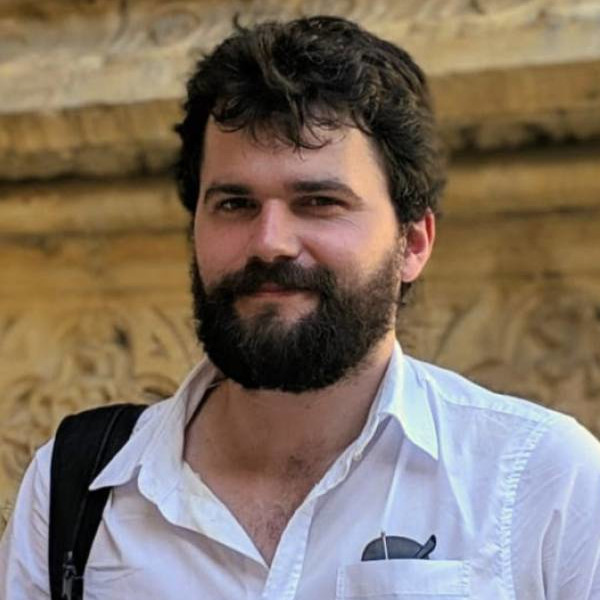
\includegraphics[height=2.0cm]{Ca_Foscari Beamer/will_handley.jpg}

\includegraphics[height=2.0cm]{Ca_Foscari Beamer/harry_bevins.jpg}
\end{center}
\eblock
\end{frame}
%This block of code is for the table of contents after
%the title page
\begin{frame}
\frametitle{Table of Contents}
\tableofcontents
\end{frame}
%---------------------------------------------------------


\section{Bayesian Inference}


% \begin{frame}{Inverse problems}\vfill

%     \begin{tikzpicture}[node distance=5cm, auto]
%     % Nodes
%     \node (params) [draw, rectangle, rounded corners, minimum width=3cm, minimum height=1cm, align=center] {model parameters \\ $\boldsymbol{\theta}$};
    
%     \node (model) [draw, rectangle, minimum width=3cm, minimum height=2cm, align=center, right of=params] {quantitative model};
    
%     \node (data) [draw, rectangle, rounded corners, minimum width=3cm, minimum height=1cm, align=center, right of=model] {data (predicted) \\ \ $\mathbf{D}$};

%      % Straight arrow with customizable height and centered text
%     \draw[->, thick] 
%     ([yshift=0cm] params.east) -- ([yshift=0cm] model.west);
    
%     \draw[->, thick] 
%     ([yshift=0cm] model.east) -- ([yshift=0cm] data.west);

%       % Text above the second rectangle
%     \node at ([yshift=0.3cm] model.north) {\textbf{Forward problem}};
%     % \draw[->, thick] 
%     % ([yshift=-0.2cm] data.west) -- node[midway, below] {\textcolor{cfred}{Inverse problem}} ([yshift=-0.2cm] model.east);

%     \node (params2) [draw, rectangle, rounded corners, minimum width=3cm, minimum height=1cm, align=center, below of=params, yshift=2cm] {model parameters, inferred \\ $\boldsymbol{\theta}_{\text{est}}$};
    
%     \node (model2) [draw, rectangle, minimum width=3cm, minimum height=2cm, align=center, below of=model, yshift=2cm] {quantitative model};

%     \node (data2) [draw, rectangle, rounded corners, minimum width=3cm, minimum height=1cm, align=center, below of=data, yshift=2cm] {data (observed) \\ \ $\mathbf{D}_\text{obs}$};

%       % Text above the second rectangle
%     \node at ([yshift=0.3cm] model2.north) {\textbf{Inverse problem}};

%      % Straight arrow with customizable height and centered text
%     \draw[->, thick, line width=1.0mm] 
%     ([yshift=0cm] params.east) -- ([yshift=0cm] model.west);
    
%     \draw[->, thick, line width=1.0mm] 
%     ([yshift=0cm] model.east) -- ([yshift=0cm] data.west);

%      % Straight arrow with customizable height and centered text
%     \draw[->, thick, line width=1.0mm] 
%     ([yshift=0cm] model2.west) -- ([yshift=0cm] params2.east);
    
%     \draw[->, thick, line width=1.0mm] 
%     ([yshift=0cm] data2.west) -- ([yshift=0cm] model2.east);


%     % % Not equal signs (≠) between vertical pairs of rectangles (ensure correct syntax for \visible)
%     \visible<2>{\node at (data -| data2) [yshift=-1.4cm] {\textcolor{red}{$\boldsymbol{\neq}$ (observational error)}};}
%     \visible<2>{\node at (params -| params2) [yshift=-1.4cm] {\textcolor{red}{$\boldsymbol{\neq}$ (error propagation)}};}
    
% \end{tikzpicture}

% \end{frame}

\begin{frame}{Inverse problems in GW physics}\vfill

    \begin{tikzpicture}[node distance=5cm, auto]
    % Nodes
    \node (params) [draw, rectangle, rounded corners, minimum width=3cm, minimum height=1cm, align=center] {model parameters \\ \textcolor{cfred}{$\boldsymbol{\theta = \mathcal{M}}\boldsymbol{,q, d_L, t_c ...}$}};
    
    \node (model) [draw, rectangle, minimum width=3cm, minimum height=2cm, align=center, right of=params] {waveform \textcolor{red}{model}};
    
    \node (data) [draw, rectangle, rounded corners, minimum width=3cm, minimum height=1cm, align=center, right of=model] {template for strain waveform \\ 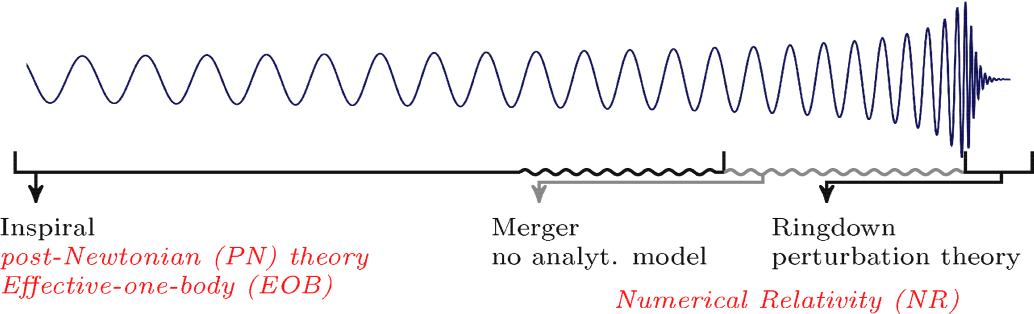
\includegraphics[width=4.2cm]{Ca_Foscari Beamer/waveform_model_inverse.png}};

     % Straight arrow with customizable height and centered text
    \draw[->, thick] 
    ([yshift=0cm] params.east) -- ([yshift=0cm] model.west);
    
    \draw[->, thick] 
    ([yshift=0cm] model.east) -- ([yshift=0cm] data.west);

      % Text above the second rectangle
    \node at ([yshift=0.3cm] model.north) {\textbf{Forward problem}};
    % \draw[->, thick] 
    % ([yshift=-0.2cm] data.west) -- node[midway, below] {\textcolor{cfred}{Inverse problem}} ([yshift=-0.2cm] model.east);

    \node (params2) [draw, rectangle, rounded corners, minimum width=3cm, minimum height=1cm, align=center, below of=params, yshift=2cm] {model parameters, inferred \\ \textcolor{cfred}{$\boldsymbol{\theta}_{\text{est}}$}};
    
    \node (model2) [draw, rectangle, minimum width=3cm, minimum height=2cm, align=center, below of=model, yshift=2cm] {\textcolor{red}{inference}};

    \node (data2) [draw, rectangle, rounded corners, minimum width=3cm, minimum height=1cm, align=center, below of=data, yshift=2cm] {observed signal strain \\ 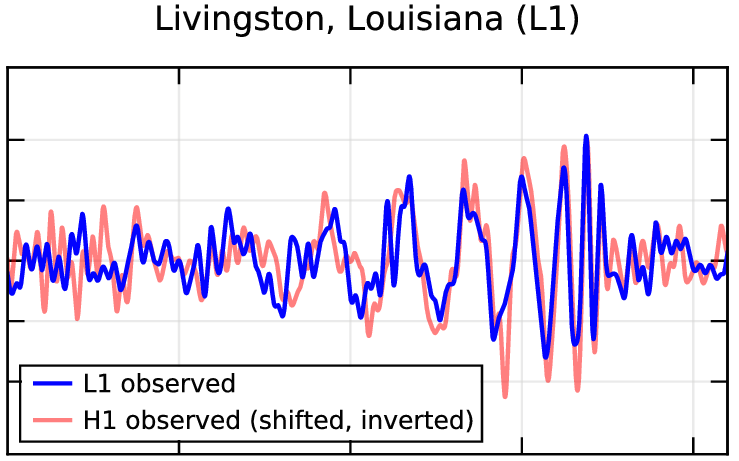
\includegraphics[width=3.5cm]{Ca_Foscari Beamer/gw_example.png.png}};

      % Text above the second rectangle
    \node at ([yshift=0.3cm] model2.north) {\textbf{Inverse problem}};

     % Straight arrow with customizable height and centered text
    \draw[->, thick, line width=1.0mm] 
    ([yshift=0cm] params.east) -- ([yshift=0cm] model.west);
    
    \draw[->, thick, line width=1.0mm] 
    ([yshift=0cm] model.east) -- ([yshift=0cm] data.west);

     % Straight arrow with customizable height and centered text
    \draw[->, thick, line width=1.0mm] 
    ([yshift=0cm] model2.west) -- ([yshift=0cm] params2.east);
    
    \draw[->, thick, line width=1.0mm] 
    ([yshift=0cm] data2.west) -- ([yshift=0cm] model2.east);


    % % Not equal signs (≠) between vertical pairs of rectangles (ensure correct syntax for \visible)
    %\visible<1>{\node at (data -| data2) [yshift=-1.4cm] {\textcolor{red}{$\boldsymbol{\neq}$ (observational error)}};}
    %\visible<1>{\node at (params -| params2) [yshift=-1.4cm] {\textcolor{red}{$\boldsymbol{\neq}$ (error propagation)}};}
    
\end{tikzpicture}

\end{frame}

% \begin{frame}{Inverse problems (cont.)}
% \begin{columns}
%     \column{0.9\textwidth}
%     \vspace{1em}
%     \centering
%     \textbf{X-ray tomography (CT)}
%     \vspace{0.5em}
%     \begin{figure}
%         \centering
%         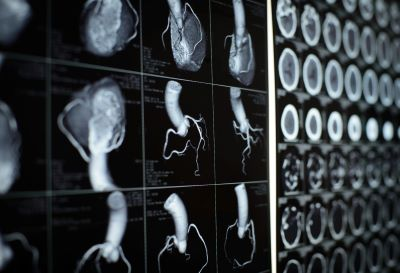
\includegraphics[width=0.3\textwidth]{Ca_Foscari Beamer/xray_tomography.jpg}
%     \end{figure}
%     \vspace{0.5em}
%     \only<1>{ 
%     \node {\textbf{Forward} : \textcolor{red}{Simulate} how X-rays pass through body.}
% }%
% \only<2>{ 
% \node {\textbf{Inverse} : Given the data (i.e. set of X-ray projections), \textcolor{red}{infer} 3D distributions of densities inside body.}
% }%
% \end{columns}
%      % General examples in the real world - reconstructing internal structure of body from X-ray or MRI data. (give what direct problem would look like.
%     % GPS - forward problem would be given your known location, calculate distances to satellites. Inverse problem is, from the signal times received from multiple satellites, infer 3D location.
%     % Speech recognition - direct probelm is given a known set of words or phonemes, model the sound waveforms they would produce. Inverse problem is, from an audio signal of speech, infer the corresponding words and phonemes. 
%     % CMB example - direct is predict CMB power spec for given model and parameters. From observed CMB data, infer parameters of LCDM.
%     % Make table to show these coming up one by one, with infer highlighted.
% \end{frame}

% \begin{frame}{Inverse problems (cont.)}
% \begin{columns}
%     \column{0.9\textwidth}
%     \vspace{1em}
%     \centering
%     \textbf{Speech recognition}
%     \vspace{0.5em}
%     \begin{figure}
%         \centering
%         
\includegraphics[width=0.3\textwidth]{Ca_Foscari Beamer/speech_recog.png}
%     \end{figure}
%     \vspace{0.5em}
%     \only<1>{ 
%     \node {\textbf{Forward} : Given a known set of words or phonemes, \textcolor{red}{model} the sound waveforms they would produce.}
% }%
% \only<2>{ 
% \node {\textbf{Inverse} : From an audio signal of speech, \textcolor{red}{infer} the corresponding words and phonemes.}
% }%
% \end{columns}
% \end{frame}


% \begin{frame}{Inverse problems (cont.)}
% \begin{columns}
%     \column{0.9\textwidth}
%     \vspace{1em}
%     \centering
%     \textbf{CMB}
%     \vspace{0.5em}
%     \begin{figure}
%         \centering
%         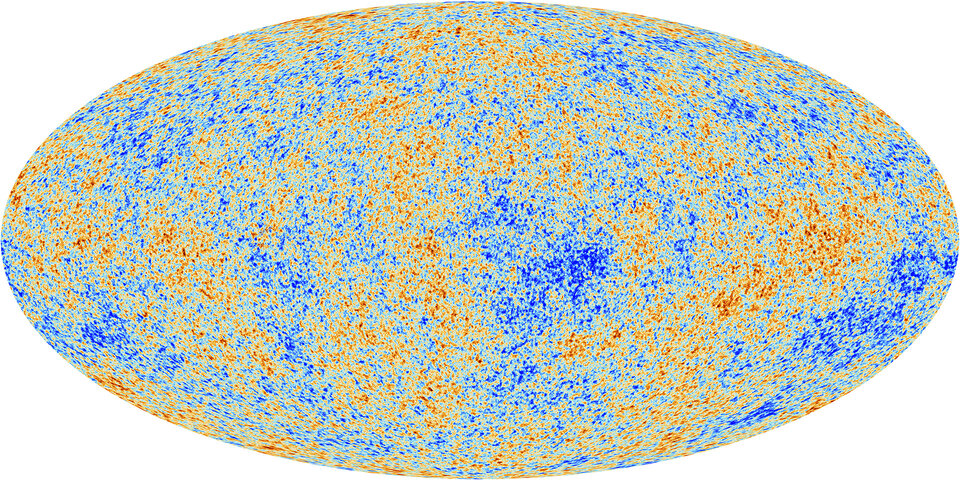
\includegraphics[width=0.3\textwidth]{Ca_Foscari Beamer/cmb.jpg}
%     \end{figure}
%     \vspace{0.5em}
%     \only<1>{ 
%     \node {\textbf{Forward} : \textcolor{red}{Predict} CMB power spectrum for given model and parameters.}
% }%
% \only<2>{ 
% \node {\textbf{Inverse} : From observed CMB data, \textcolor{red}{infer} parameters of LCDM.}
% }%
% \end{columns}
% \end{frame}

%-------------------------------------------------------------
% \begin{frame}{Inverse problems in GW physics}
% \begin{columns}
%     \column{0.9\textwidth}
%     \vspace{1em}
%     \centering
%     \textbf{GW astronomy}
%     \vspace{0.5em}
%     \begin{figure}
%         \centering
%         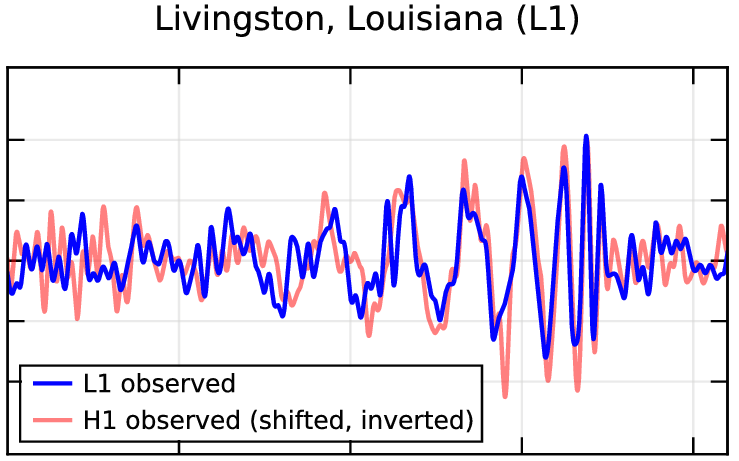
\includegraphics[width=0.3\textwidth]{Ca_Foscari Beamer/gw_example.png.png}
%     \end{figure}
%     \vspace{0.5em}
%     \only<1>{ 
%     \node {\textbf{Forward} : Given a waveform model and a set of binary parameters, \textcolor{red}{model} the GW signal.}
% }%
% \only<2>{ 
% \node {\textbf{Inverse} : From an observed signal strain, $h(t)$, \textcolor{red}{infer} the binary parameters (e.g. masses, spins, luminosity distance, sky location etc.)}
% }%
% \end{columns}
% \end{frame}

\begin{frame}{Deterministic approach}
\begin{itemize}
    \item One naive way to tackle this is to directly fit the waveform model to the data by minimizing the differences between the two.
    \item Produces a single set of best-fit parameters.
\end{itemize}
\vspace{2em}
Issues:
\begin{itemize}
    \item \textbf{Degenerate solutions} - different combinations of parameters can produce near-identical signals (e.g. mass spin degeneracy).
    \item \textbf{Noisy data} - can lead to biased parameter estimates.
\end{itemize}
\end{frame}

\begin{frame}{Probabilistic approach}\vfill
\begin{itemize}
    \item Instead of single ``best-fit'' solution, obtain \textbf{posterior distribution} over possible parameters.
\end{itemize}
\vspace{0cm}
\begin{minipage}{0.4\textwidth}
    \centering
    $\{m_1, m_2\}^\text{best-fit} = \{36.3, 28.6\}$
\end{minipage}%
\hspace{0.25\textwidth} % Adjust spacing between the minipages
\begin{minipage}{0.3\textwidth}
    \centering
    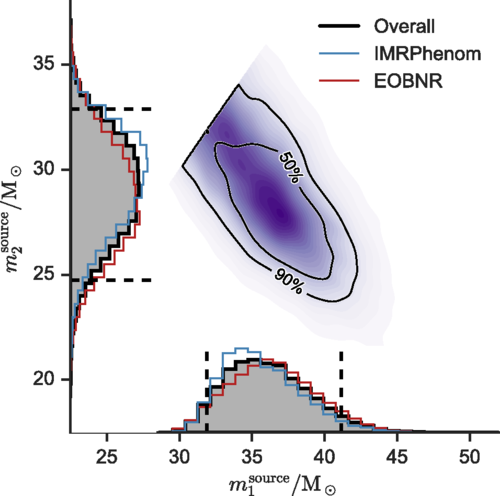
\includegraphics[width=0.6\textwidth]{Ca_Foscari Beamer/posteriors.png}
\end{minipage}
\begin{tikzpicture}[overlay]
    \draw[->, thick] (-7, 0) -- (-5, 0); % Adjust coordinates to match the minipages
\end{tikzpicture}
\begin{itemize}
    \item Accounts for uncertainty in data and model.
    \item Even in the presence of noise or degeneracies, provides a complete probabilistic picture of parameter estimates.
\end{itemize}\vfill
Bayesian inference provides a robust framework for doing this!
\end{frame}
%---------------------------------------------------------
%Changing visibility of the text
\begin{frame}{Bayes' Theorem}

Given some model $\mathcal{M}$ and observed signal $\mathcal{D}$, Bayes' theorem enables us to relate the \textcolor{RoyalBlue}{posterior} probability of the set of parameters $\theta$ which generated the signal to the \textcolor{Purple}{likelihood} of the $\mathcal{D}$ given $\theta$ and the \textcolor{BurntOrange}{prior} probability of $\theta$ given $\mathcal{M}$:
\vfill
\begin{equation}
    \textcolor{RoyalBlue}{\mathcal{P}(\theta | D, \mathcal{M})} = \frac{\textcolor{Purple}{P(D | \theta, \mathcal{M})} \textcolor{BurntOrange}{P(\theta | \mathcal{M})}}{\textcolor{red}{P(D | \mathcal{M})}} = \frac{\textcolor{Purple}{\mathcal{L}(D | \theta)} \textcolor{BurntOrange}{\pi(\theta)}}{\textcolor{red}{\mathcal{Z}}}
\end{equation}
\vfill
The \textcolor{red}{evidence}, \textcolor{red}{$\mathcal{Z}$}, plays a key role in model comparison.
\end{frame}

\begin{frame}{Bayesian inference}
\begin{columns}
    
\column{0.5\textwidth}
\begin{itemize}
    \item Define \textcolor{BurntOrange}{prior}, \textbf{sample} (unnormalized) \textcolor{RoyalBlue}{posterior} ($\mathcal{L}(D | \theta) \times \pi(\theta)$).
    % \item Cannot plot full posterior distribution but can plot 1D and 2D \textbf{marginal} distributions (e.g. $\mathcal{P}(\mathcal{M}, q, \chi_\text{eff} | D)$) by integrating over all other parameters.
\end{itemize}
\vspace{2em}
\raggedright
Challenges:\vfill
    \begin{itemize}
        \item High-dimensional parameter spaces $\Rightarrow$ \textcolor{RoyalBlue}{posterior} occupies vanishingly small region of \textcolor{BurntOrange}{prior}.
        \item Complex likelihoods with high costs
    \end{itemize}
    \vfill 

\column{0.5\textwidth}\
\vspace{-2em}
\centering
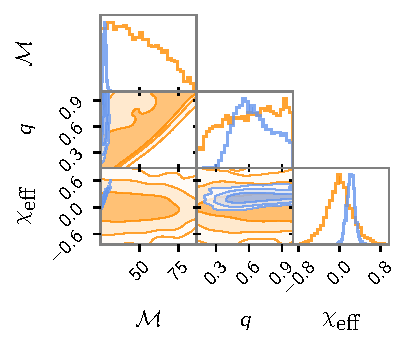
\includegraphics[]{Ca_Foscari Beamer/presentation_triangleplot.pdf}
\end{columns}
\end{frame}

% \begin{frame}{Sampling}

%     Challenges:\vfill
%     \begin{itemize}
%         \item High-dimensional parameter spaces $\Rightarrow$ posterior occupies vanishingly small region of prior.
%         \item Complex likelihoods with high costs
%     \end{itemize}
%     \vfill 
    
%     Goal is efficient exploration of parameter space, so need more sophisticated sampling methods to do GW inference in feasible timescales. 

%     % Goal : efficient exploration of parameter space. 
%     % Sampling: allows us to approximate distributions from discrete points.
%     % Sampling is process of drawing discrete points from a prob dist such that density of points reflects shape of dist. By drawing enough points, can approximate trye shape of posterior. 
%     % Can sample randomly but inefficient for high dimensional problems.
%     % Two main approaches: MCMC methods and nested sampling.
% \end{frame}

\begin{frame}{Samplers}\vfill
Goal is efficient exploration of parameter space, to do GW inference in feasible timescales. 
\vfill  
    \textcolor{RoyalBlue}{Posterior} samplers:
    \begin{itemize}
        \item Metropolis-Hastings 
        \item Hamiltonian Monte-Carlo
        \item Ensemble samplers
    \end{itemize}
    \vfill
    None of these calculate the \textcolor{red}{evidence}, \textcolor{red}{$\mathcal{Z}$} - crucial for Bayesian model comparison (e.g. testing for precession vs. no precession)!

    
\end{frame}

\section{Nested sampling}

%---------------------------------------------------------
\begin{frame}
\frametitle{Evidence}
Nested sampling first and foremost calculates this \textcolor{red}{evidence}. The \textcolor{red}{evidence} is the integral of likelihood $\times$ prior over the entire parameter space,
\begin{equation}
    \textcolor{red}{\mathcal{Z}} = \int \mathcal{L(\theta)} \pi(\theta) d\theta,
\end{equation}
which, in general, is a many dimensional integral.
\vfill

NS turn this into a 1D problem, performing this integral by summing over nested likelihood contours in the parameter space.
\end{frame}

% \begin{frame}{Outputs in \textsc{bilby}}
%     \begin{minipage}[]{0.5\textwidth}
%     \centering
%         \includegraphics[width=0.95\textwidth]{Ca_Foscari Beamer/bilby_\textcolor{red}{evidence}.png}
%     \end{minipage}%
%     \begin{minipage}[]{0.5\textwidth} \vspace{2em}
%         \centering
%         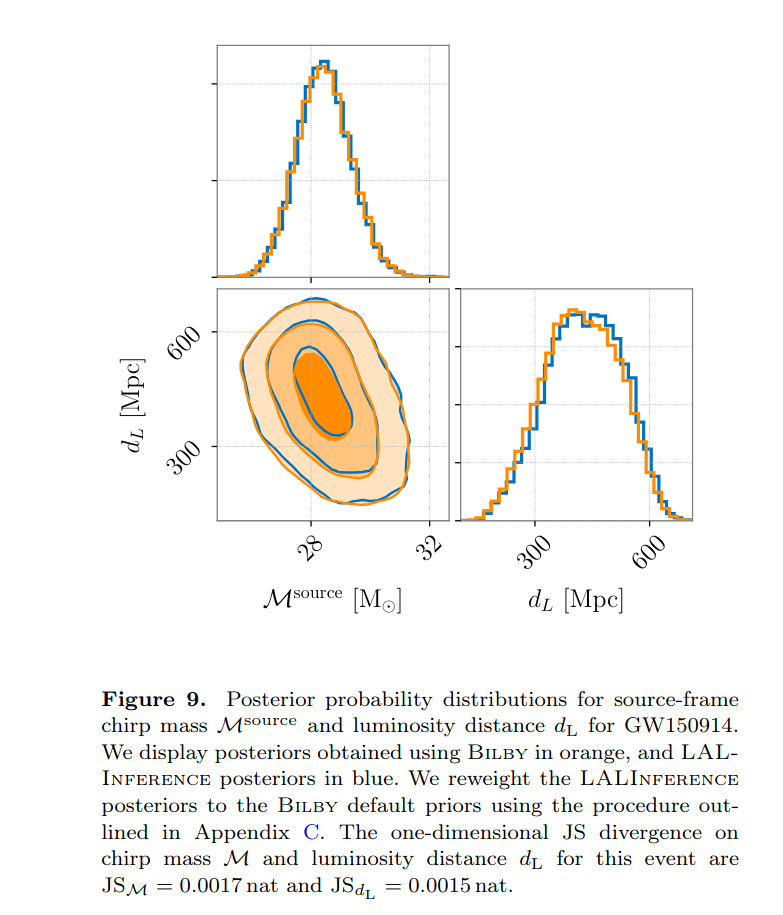
\includegraphics[width=0.75\textwidth]{Ca_Foscari Beamer/bilby_triangle.png}
%     \end{minipage}
%   \textcolor{cfgrey}{2006.00714}
% \end{frame}

%---------------------------------------------------------
%Example of the \pause command
\begin{frame}
\frametitle{Nested sampling (NS)}\vfill
Nested sampling first and foremost calculates \textcolor{red}{evidence}, $\textcolor{red}{\mathcal{Z}} = \int \mathcal{L(\theta)} \pi(\theta) d\theta$.
\begin{minipage}[]{0.35\textwidth}
\vspace{20em}
\visible<1>{
\begin{tikzpicture}
\def\svgwidth{\textwidth}
\input{NS_cartoon_2.pdf_tex}
\end{tikzpicture}
}
\visible<2>{
\begin{tikzpicture}
\def\svgwidth{\textwidth}
\hspace{-0.39cm}
\input{NS_cartoon_3.pdf_tex}
\end{tikzpicture}
}
\visible<3>{
\begin{tikzpicture}
\def\svgwidth{\textwidth}
\hspace{-0.78cm}
\input{NS_cartoon_4.pdf_tex}
\end{tikzpicture}
}
\visible<4>{
\begin{tikzpicture}
\def\svgwidth{\textwidth}
\hspace{-1.2cm}
\input{NS_cartoon_5.pdf_tex}
\end{tikzpicture}
}
\visible<5>{
\begin{tikzpicture}
\def\svgwidth{\textwidth}
\hspace{-1.6cm}
\input{NS_cartoon_5.pdf_tex}
\end{tikzpicture}
}
\vspace{-5em}
\end{minipage}\hfill
\begin{minipage}{0.5\textwidth}
    \begin{itemize}
        \item<1-> Prior is populated with set of `live points'.
        \item<2-> At each iteration $i$, point is lowest likelihood is deleted and new live point is drawn, which must have a likelihood higher than that of the deleted point.
        \item<4-> Live points compress exponentially towards peak of likelihood.
        \item<5-> \textcolor{red}{Evidence} is calculated as weighted sum over deleted (`dead') points.
    \end{itemize}
    %\vspace{-2.5em}
\end{minipage}
\end{frame}

% \begin{frame}{Outputs in \textsc{bilby}}
%     \begin{minipage}[]{0.5\textwidth}
%     \centering
%         \includegraphics[width=0.95\textwidth]{Ca_Foscari Beamer/bilby_\textcolor{red}{evidence}.png}
%     \end{minipage}%
%     \begin{minipage}[]{0.5\textwidth} \vspace{2em}
%         \centering
%         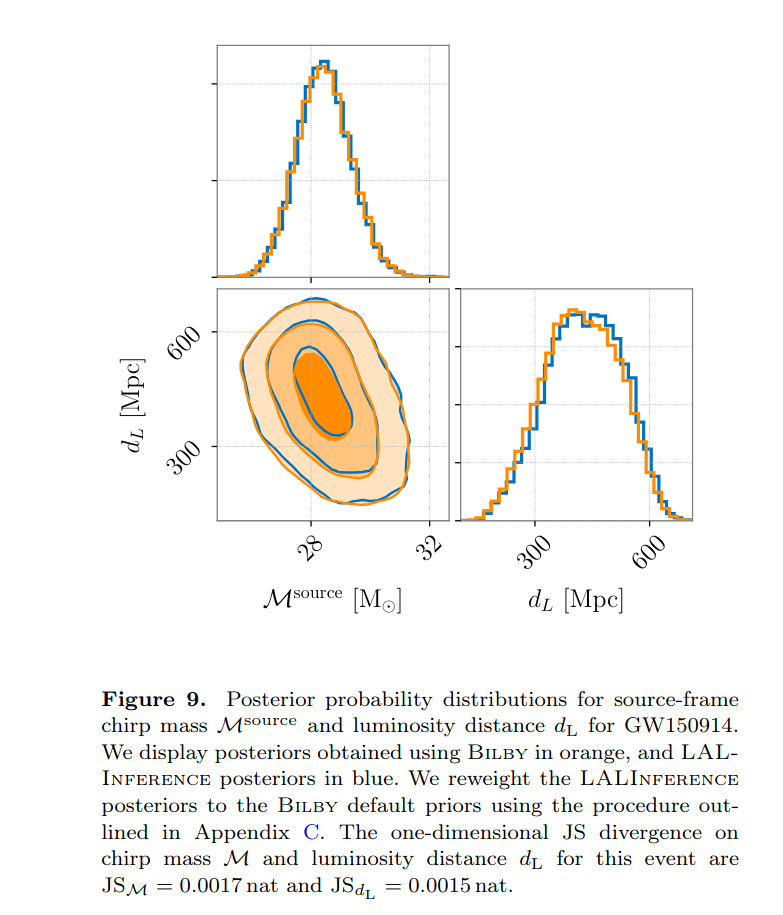
\includegraphics[width=0.75\textwidth]{Ca_Foscari Beamer/bilby_triangle.png}
%     \end{minipage}
%   \textcolor{cfgrey}{2006.00714}
% \end{frame}

\begin{frame}{Drawing new live point}
\begin{itemize}
    \item This is not trivial!
    \item Different samplers implement this step in different ways, but most samplers can broadly be split into 2 categories:
\end{itemize}
\begin{enumerate}
    \item Region samplers (e.g. \textsc{MultiNest}, \textsc{nessai}, \textsc{UltraNest})
    \begin{itemize}
        \item Construct a bounding region for the deleted point's likelihood contour and sample within this.
        \item Generates invalid points that have to be discarded.
    \end{itemize}
    \item Path samplers (e.g. \textsc{PolyChord}, \textsc{CPNest}, \textsc{dynesty})
    \begin{itemize}
        \item Run a Markov chain from the deleted point.
        \item Generates correlated (but valid) points that have to be discarded.
    \end{itemize}
\end{enumerate}
    % Not trivial. Broadly can split many NS algos into two categories for how they do this. (rejection vs chain-based).
    % Other approached exist (importance samplers, nessai, etc. - research!!)
\end{frame}

\begin{frame}{KL divergence}
\vspace{3em}
\begin{itemize}
    \item The Kullback Liebler divergence between the \textcolor{BurntOrange}{prior} and \textcolor{RoyalBlue}{posterior} is defined as:
\end{itemize}

\begin{equation}
    \mathcal{D}_\text{KL} = \left\langle \text{log} \frac{\mathcal{P}}{\pi} \right\rangle_\mathcal{P} \approx \text{log}\frac{V_\mathcal{P}}{V_\pi}
\end{equation}

\begin{itemize}
    \item ``Amount of compression from \textcolor{BurntOrange}{prior} to \textcolor{RoyalBlue}{posterior}''
\end{itemize}%
\begin{minipage}{0.8\textwidth}\vspace{21em}
    \begin{tikzpicture}
    \def\svgwidth{0.5\textwidth}
    \hspace{10em}
    \input{PR_cartoon.pdf_tex}
    \end{tikzpicture}
\end{minipage}

    % Slide on KL divergence - what is it? How is it calculated? How is it relevant for NS?
\end{frame}

%---------------------------------------------------------

\section{Accelerating NS}

%---------------------------------------------------------
%Highlighting text
% \begin{frame}{Runtime of NS}
% Time of convergence of NS:
% \vfill
%     \begin{equation}
%         T \propto \tikzmarknode{a1}{T_{\mathcal{L}}} \times \tikzmarknode{a2}{f_{\textrm{sampler}}} \times \visible<2->{\tikz\node[draw=cfred, inner sep=8.5pt, circle, overlay, shift={(10pt,2pt)}]{}} \tikzmarknode{a3}{D_{\textrm{KL}}} \times \tikzmarknode{a4}{n_{\textrm{live}}} 
%     \end{equation}
%     \begin{tikzpicture}[remember picture, overlay]
%     \visible<6>{\draw[explain, <-, thick, cfred](a4)--++(1.5,2)node[above]{resolution};}
%     \visible<4-7>{\draw[explain, <-, thick, cfred](a1)--++(-1,-0.9)node[below]{single likelihood evaluation time};}
%     \visible<5-8>{\draw[explain, <-, thick, cfred](a2)--++(-2,1)node[above]{drawing new live point subject to hard likelihood constraint};}
%     \visible<5>{}
%     \visible<3-9>{\draw[explain, <-, thick, cfred](a3)--++(.5,-2)node[below]{compression from prior to posterior ($\approx \mathrm{ln}\frac{V_\pi}{V_\mathcal{P}}$)};}
%     \visible<7->{\draw[explain, <-, thick](a4)--++(1.5,2)node[above]{resolution (baked in)};}
%     \visible<8->{\draw[explain, <-, thick](a1)--++(-1,-0.9)node[below]{faster waveform models};}
%      \visible<9->{\draw[explain, <-, thick](a2)--++(-2,1)node[above]{better samplers};}
%      \visible<2>{\draw[explain, <-, thick, cfred](a3)--++(.5,-2)node[below]{focus of this talk};}
%     \end{tikzpicture}
% \end{frame}

% \begin{frame}{Runtime of NS}
%     %Time of convergence of NS:

% \begin{equation}
%     T \propto \tikzmarknode{Tl}{T_\mathcal{L}} \times \tikzmarknode{nl}{\only<1>{n_\mathcal{L}}} \tikzmarknode{fsampler}{\visible<2->{f_\textrm{sampler}}} \visible<2->{\times}  \tikzmarknode{niter}{\only<2>{n_\textrm{iter}}}  \visible<4>{\tikz\node[draw=cfred, inner sep=8.5pt, circle, overlay, shift={(10pt,2pt)}]{}}  \tikzmarknode{DKL}{\visible<3->{\mathcal_{D}_{\mathrm{KL}}}} \visible<3->{\times} \tikzmarknode{nlive}{\visible<3->{n_\textrm{live}}} 
% \end{equation}
% \begin{tikzpicture}[remember picture, overlay]
%     \visible<1->{\draw[explain, <-, thick, cfred] (Tl)--++(-2,1) 
%     node[above]{likelihood evaluation time};}
%     \visible<1>{\draw[explain, <-, thick, cfred] (nl)--++(2,-1) 
%     node[below]{number of likelihood evaluations};}
%     \visible<2->{\draw[explain, <-, thick, cfred] (fsampler)--++(-2.5,-1.5) 
%     node[below]{number of likelihood evaluations per iteration};}

%     \visible<2->{\node[anchor=south, inner sep=12pt] at (current page.south west) {\hspace{8em}
%         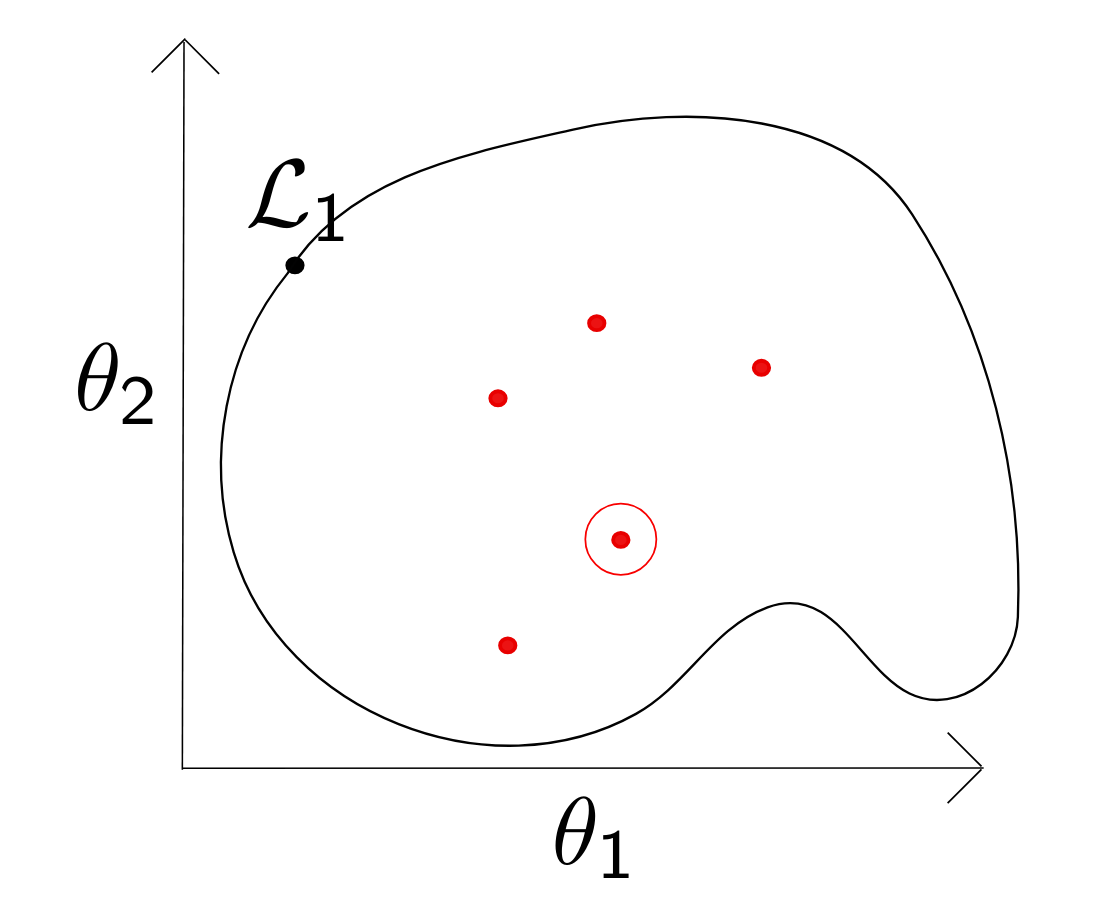
\includegraphics[width=0.2\textwidth]{Ca_Foscari Beamer/Screenshot from 2024-11-22 10-06-12.png}
%     };
%     }

%     \visible<2>{\draw[explain, <-, thick, cfred] (niter)--++(1,1) 
%     node[above]{number of iterations};}

%     \visible<3>{\draw[explain, <-, thick, cfred] (DKL)--++(2,-0.7) 
%     node[below]{compression between prior and posterior ($\approx \mathrm{log}\frac{V_\pi}{V_\mathcal{P}}$)};}

%     \visible<3->{\draw[explain, <-, thick, cfred] (nlive)--++(1,1) 
%     node[above]{resolution};}

%     \visible<4>{\draw[explain, <-, ultra thick, cfred] (DKL)--++(2,-0.7) 
%     node[below]{focus of this talk!};}
    
% \end{tikzpicture}

% \end{frame}

\begin{frame}{Runtime of NS}

    \begin{equation}
        T \propto 
        \tikzmarknode{Tl}{T_\mathcal{L}} 
        \times 
        \tikzmarknode{nl}{\onslide<1>{n_\mathcal{L}}} 
        \tikzmarknode{fsampler}{\onslide<2->{\hspace*{-1.1em}f_\textrm{sampler}}} 
        \onslide<2->{\times}  
        \tikzmarknode{niter}{\onslide<2>{n_\textrm{iter}}}  
        \onslide<4->{\tikz\node[draw=cfred, inner sep=8.5pt, circle, overlay, shift={(-8pt,2pt)}]{}}  
        \tikzmarknode{DKL}{\onslide<3->{\hspace*{-1.6em} \mathcal{D}_{\mathrm{KL}}}} 
        \onslide<3->{\times} 
        \tikzmarknode{nlive}{\onslide<3->{n_\textrm{live}}} 
    \end{equation}
    \begin{tikzpicture}[remember picture, overlay]
        \onslide<1->{\draw[explain, <-, thick, cfred] (Tl)--++(-2,1) 
        node[above]{likelihood evaluation time};}

        \onslide<1>{\draw[explain, <-, thick, cfred] (nl)--++(2,-1) 
        node[below]{number of likelihood evaluations};}

        \onslide<2->{\draw[explain, <-, thick, cfred] (fsampler)--++(-3,-1.7) 
        node[below]{drawing new live point};}

        \onslide<2->{\node[anchor=south, inner sep=12pt] at (current page.south west) {\hspace{8em}
            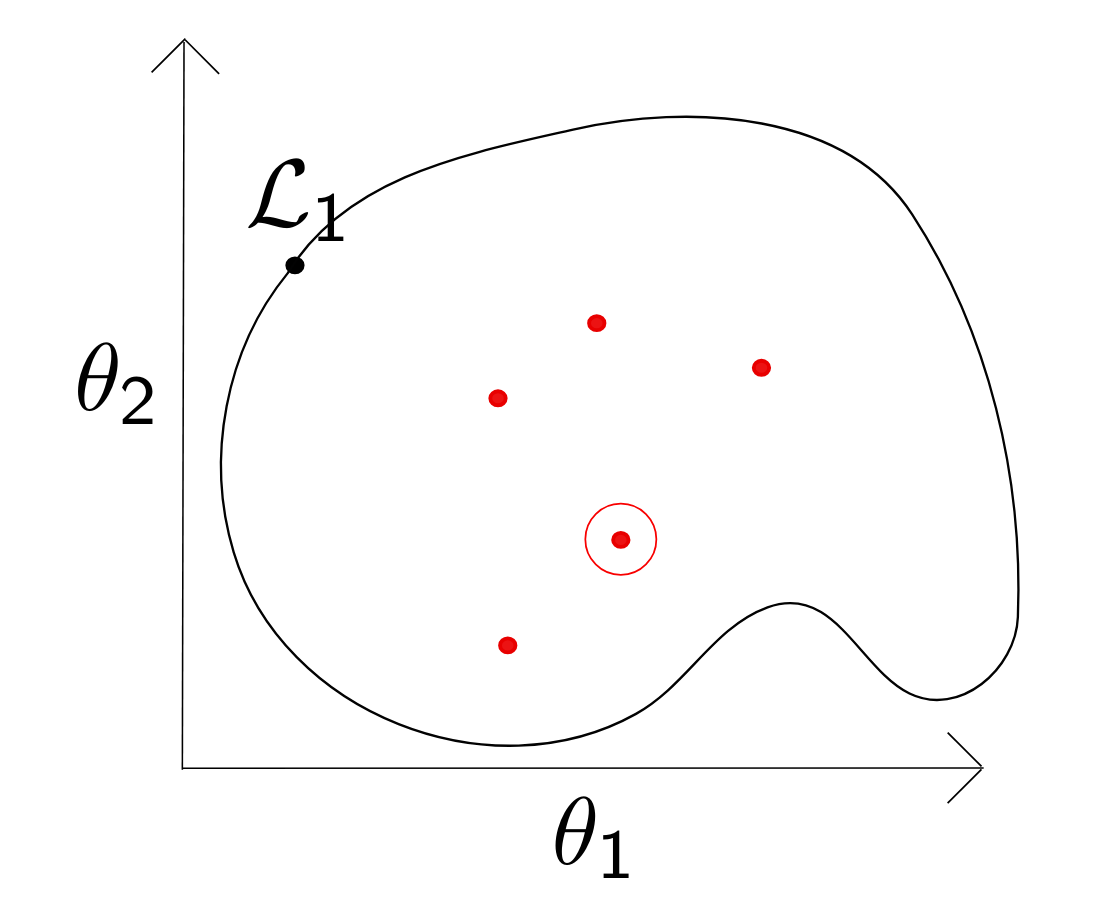
\includegraphics[width=0.2\textwidth]{Ca_Foscari Beamer/Screenshot from 2024-11-22 10-06-12.png}
        };}

        \onslide<2>{\draw[explain, <-, thick, cfred] (niter)--++(1,1) 
        node[above]{number of iterations};}

        \onslide<3>{\draw[explain, <-, thick, cfred] (DKL)--++(1.2,-0.8) 
        node[below]{compression between \textcolor{BurntOrange}{prior} and \textcolor{RoyalBlue}{posterior} ($\approx \mathrm{log}\frac{V_\pi}{V_\mathcal{P}}$)};}

        \onslide<3->{\draw[explain, <-, thick, cfred] (nlive)--++(1,1) 
        node[above]{resolution};}

        \onslide<4>{\draw[explain, <-, ultra thick, cfred] (DKL)--++(1.2,-0.8) 
        node[below]{focus of this talk!};}
    \end{tikzpicture}
\end{frame}


\begin{frame}{Accelerating NS}

    % \begin{equation}
    %     T \propto 
    %     \tikzmarknode{Tl}{T_\mathcal{L}} 
    %     \times 
    %     \tikzmarknode{fsampler}{\onslide<1->{f_\textrm{sampler}}} 
    %     \onslide<1->{\times}   
    %     \onslide<1->{\tikz\node[draw=cfred, inner sep=8.5pt, circle, overlay, shift={(10pt,2pt)}]{}}  
    %     \tikzmarknode{DKL}{\onslide<1->{\mathcal{D}_{\mathrm{KL}}}} 
    %     \onslide<1->{\times} 
    %     \tikzmarknode{nlive}{\onslide<1->{n_\textrm{live}}} 
    % \end{equation}
    \begin{equation}
        T \propto 
        \tikzmarknode{Tl}{T_\mathcal{L}} 
        \times 
        \tikzmarknode{nl}{\onslide<1>{\textcolor{white}{n_\mathcal{L}}}} 
        \tikzmarknode{fsampler}{\onslide<1->{\hspace*{-1.1em}f_\textrm{sampler}}} 
        \onslide<1->{\times}  
        \tikzmarknode{niter}{\onslide<1>{\textcolor{white}{n_\textrm{iter}}}}  
        \onslide<1->{\tikz\node[draw=cfred, inner sep=8.5pt, circle, overlay, shift={(-8pt,2pt)}]{}}  
        \tikzmarknode{DKL}{\onslide<1->{\hspace*{-1.6em} \mathcal{D}_{\mathrm{KL}}}} 
        \onslide<1->{\times} 
        \tikzmarknode{nlive}{\onslide<1->{n_\textrm{live}}} 
    \end{equation}
    \begin{tikzpicture}[remember picture, overlay]
        \onslide<1-2>{\draw[explain, <-, thick, cfred] (Tl)--++(-2,1) 
        node[above]{likelihood evaluation time};}
        \onslide<3->{\draw[explain, <-, thick, black] (Tl)--++(-2,1) 
        node[above]{faster waveform models};}

        \onslide<1-3>{\draw[explain, <-, thick, cfred] (fsampler)--++(-3,-1.7) 
        node[below]{drawing new live point};}
        \onslide<4->{\draw[explain, <-, thick, black] (fsampler)--++(-3,-1.7) 
        node[below]{better samplers};}

        \onslide<1->{\node[anchor=south, inner sep=12pt] at (current page.south west) {\hspace{8em}
            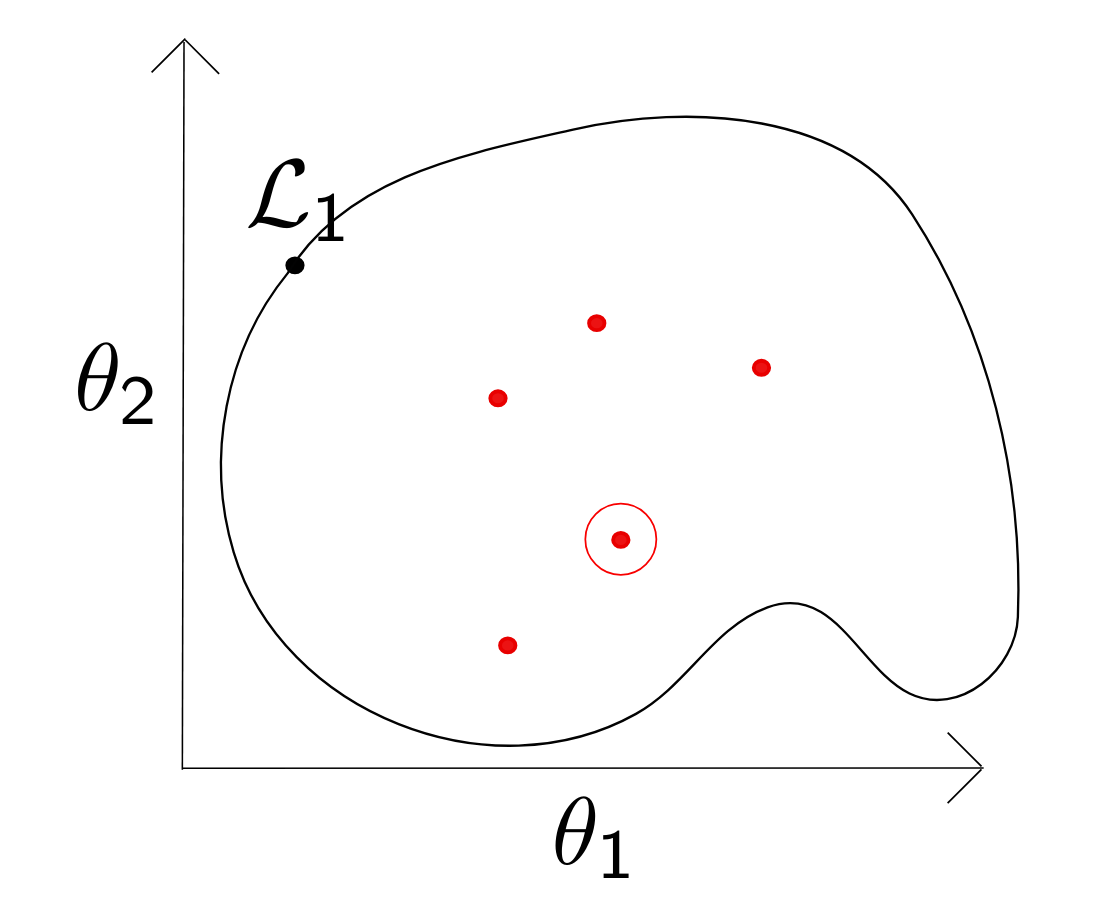
\includegraphics[width=0.2\textwidth]{Ca_Foscari Beamer/Screenshot from 2024-11-22 10-06-12.png}
        };}

        \onslide<1->{\draw[explain, <-, thick, cfred] (DKL)--++(1.2,-0.8) 
        node[below]{compression between \textcolor{BurntOrange}{prior} and \textcolor{RoyalBlue}{posterior} ($\approx \mathrm{log}\frac{V_\pi}{V_\mathcal{P}}$)};}

        \onslide<1>{\draw[explain, <-, thick, cfred] (nlive)--++(1,1) 
        node[above]{resolution};}
        \onslide<2->{\draw[explain, <-, thick, black] (nlive)--++(1,1) 
        node[above]{resolution (baked in)};}
    \end{tikzpicture}
\end{frame}

% \begin{frame}{Accelerating NS}

% %\vfill
% \begin{equation}
%     T \propto \tikzmarknode{a1}{T_{\mathcal{L}}} \times \tikzmarknode{a2}{f_{\textrm{sampler}}} \times 
%     \visible<1->{\tikz\node[draw=cfred, inner sep=8.5pt, circle, overlay, shift={(10pt,2pt)}]{}} 
%     \tikzmarknode{a3}{D_{\textrm{KL}}} \times \tikzmarknode{a4}{n_{\textrm{live}}} 
% \end{equation}
% \begin{tikzpicture}[remember picture, overlay]
%     % T_L annotation
%     \visible<1-2>{\draw[explain, <-, thick, cfred] (Tl)--++(-2,1) 
%     node[above]{likelihood evaluation time};}
%     \visible<3->{\draw[explain, <-, thick] (a1)--++(-2,1) 
%     node[above]{faster waveform models};}%
%     % f_sampler annotation
%      % Adding the image for the arrow description
%     \visible<1->{\node[anchor=south, inner sep=12pt] at (current page.south west) {\hspace{8em}
%         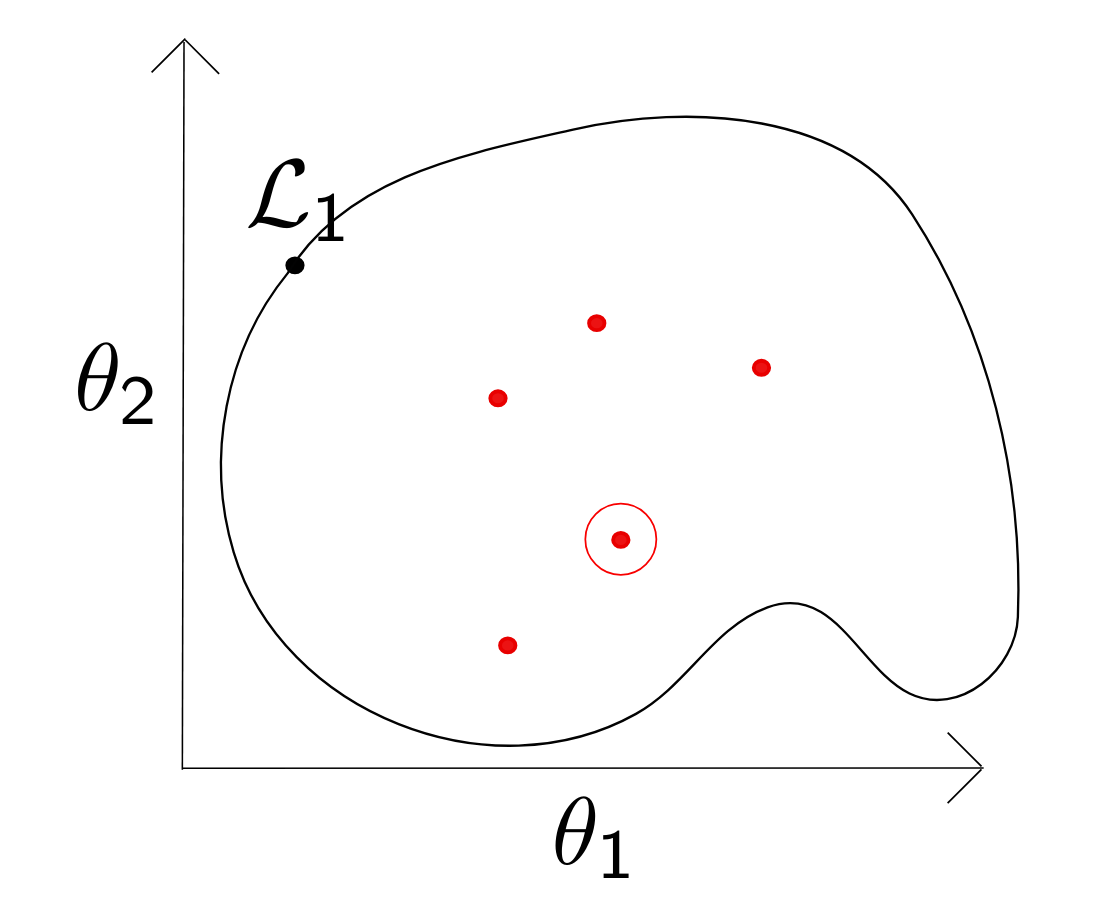
\includegraphics[width=0.2\textwidth]{Ca_Foscari Beamer/Screenshot from 2024-11-22 10-06-12.png}
%     };
%     }%
%     \visible<1-3>{\draw[explain, <-, thick, cfred] (fsampler)--++(-2.5,-1.5) 
%     node[below]{drawing a new live point};}%
%     \visible<4->{\draw[explain, <-, thick] (a2)--++(-2.5,-1.5) 
%     node[below]{better samplers};}
    
%     % D_KL annotation
%     \visible<1->{\draw[explain, <-, thick, cfred] (DKL)--++(2,-0.7) 
%     node[below]{compression between prior and posterior ($\approx \mathrm{log}\frac{V_\pi}{V_\mathcal{P}}$)};}
%     % \visible<1>{\draw[explain, <-, ultra thick, cfred] (a3)--++(.5,-2) 
%     % node[below]{focus of this talk};}

%     % n_live annotation
%     \visible<1>{\draw[explain, <-, thick, cfred](a4)--++(1,1)node[above]{resolution};}
%     \visible<2->{\draw[explain, <-, thick] (a4)--++(1,1) 
%     node[above]{resolution (baked in)};}
% \end{tikzpicture}
% \end{frame}

\begin{frame}{Uncertainty of NS}

\begin{block}{Time of convergence of NS}
    \begin{equation}
        T \propto T_{\mathcal{L}} \times f_{\textrm{sampler}} \times D_{\textrm{KL}} \times n_{\textrm{live}} 
    \end{equation}
\end{block}
\begin{block}{Uncertainty in log$\textcolor{red}{\mathcal{Z}}$}
    \begin{equation}
        \sigma \propto \sqrt{D_{\textrm{KL}} / n_{\textrm{live}}}
    \end{equation}
\end{block}

\alert{Precision-normalized} runtime has quadratic dependence on KL divergence. \textcolor{cfgrey}{2212.01760}
    
\end{frame}

\begin{frame}{REACH}
\vspace{2em}
One way to do this (REACH):
\vfill
\centering
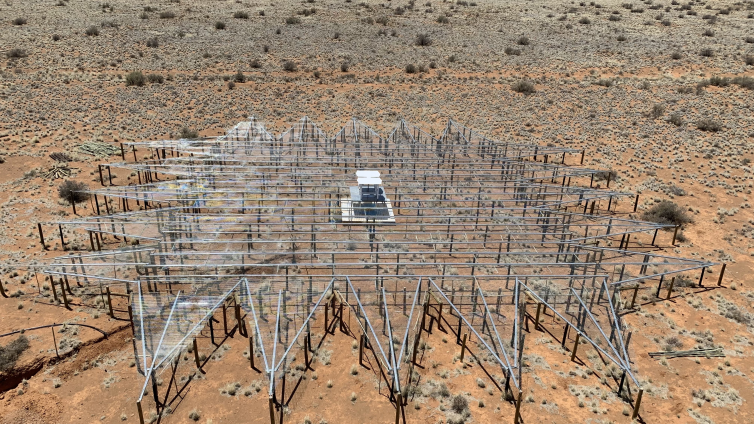
\includegraphics[width=0.6\textwidth]{Ca_Foscari Beamer/antenna.png}

\end{frame}

\begin{frame}{Reducing $D_{\textrm{KL}}$}
\vspace{3.5em}
One way to do this (REACH):

\begin{minipage}[]{0.45\textwidth}\vspace{22em}
%\includegraphics<1>[0.9\textwidth]{Ca_Foscari Beamer/antenna.png}%
\visible<1>{
\begin{tikzpicture}
\def\svgwidth{0.9\textwidth}
\input{PR_cartoon.pdf_tex}
\end{tikzpicture}
}
\visible<2>{
\begin{tikzpicture}
\def\svgwidth{0.9\textwidth}
\hspace{-0.96em}
\input{PR_cartoon_2.pdf_tex}
\end{tikzpicture}
}
\visible<3>{
\begin{tikzpicture}
\def\svgwidth{0.9\textwidth}
\hspace{-2em}
\input{PR_cartoon_3.pdf_tex}
\end{tikzpicture}
}
\end{minipage}
\begin{minipage}{0.45\textwidth}\vspace{-8em}
\begin{itemize}
    \item<1-> Perform low resolution (low live points) run first to roughly identify where \textcolor{RoyalBlue}{posterior} lies.
    \item<2-> Then set off second, high resolution, run with \textbf{narrower} box \textcolor{BurntOrange}{prior} (much quicker).
    \item<3-> \textcolor{red}{Evidence} has \textbf{changed} (since different prior), but easy to correct (multiply new evidence by $\frac{V_{\pi^\ast}}{V_\pi}$)
\end{itemize}
\end{minipage}

\end{frame}


\begin{frame}{When does this break down?}\vspace{33em}
\begin{minipage}{0.6\textwidth}
   \begin{tikzpicture}
   \centering
       \def\svgwidth{\textwidth}
       \hspace{-2em}
        \input{PR_cartoon_banana.pdf_tex}
   \end{tikzpicture}
\end{minipage}
\begin{minipage}{0.3\textwidth}\vspace{-45em}
\begin{itemize}
    \item Banana distributions, multi-modality etc.
    \item Precludes its use in most realistic GW cases...
\end{itemize}
\end{minipage}
\end{frame}

\begin{frame}{NFs}
    \begin{itemize}\vspace{3em}

    \item<1-> Can iterate on this by using \textbf{normalizing flows} (NF) to learn the rough \textcolor{RoyalBlue}{posterior}.
    \item<2-> NFs perform density estimation, by learning a series of invertible mappings from the standard normal distribution to the target (posterior). 
\end{itemize}\vspace{0em}
    \visible<2->{\centering 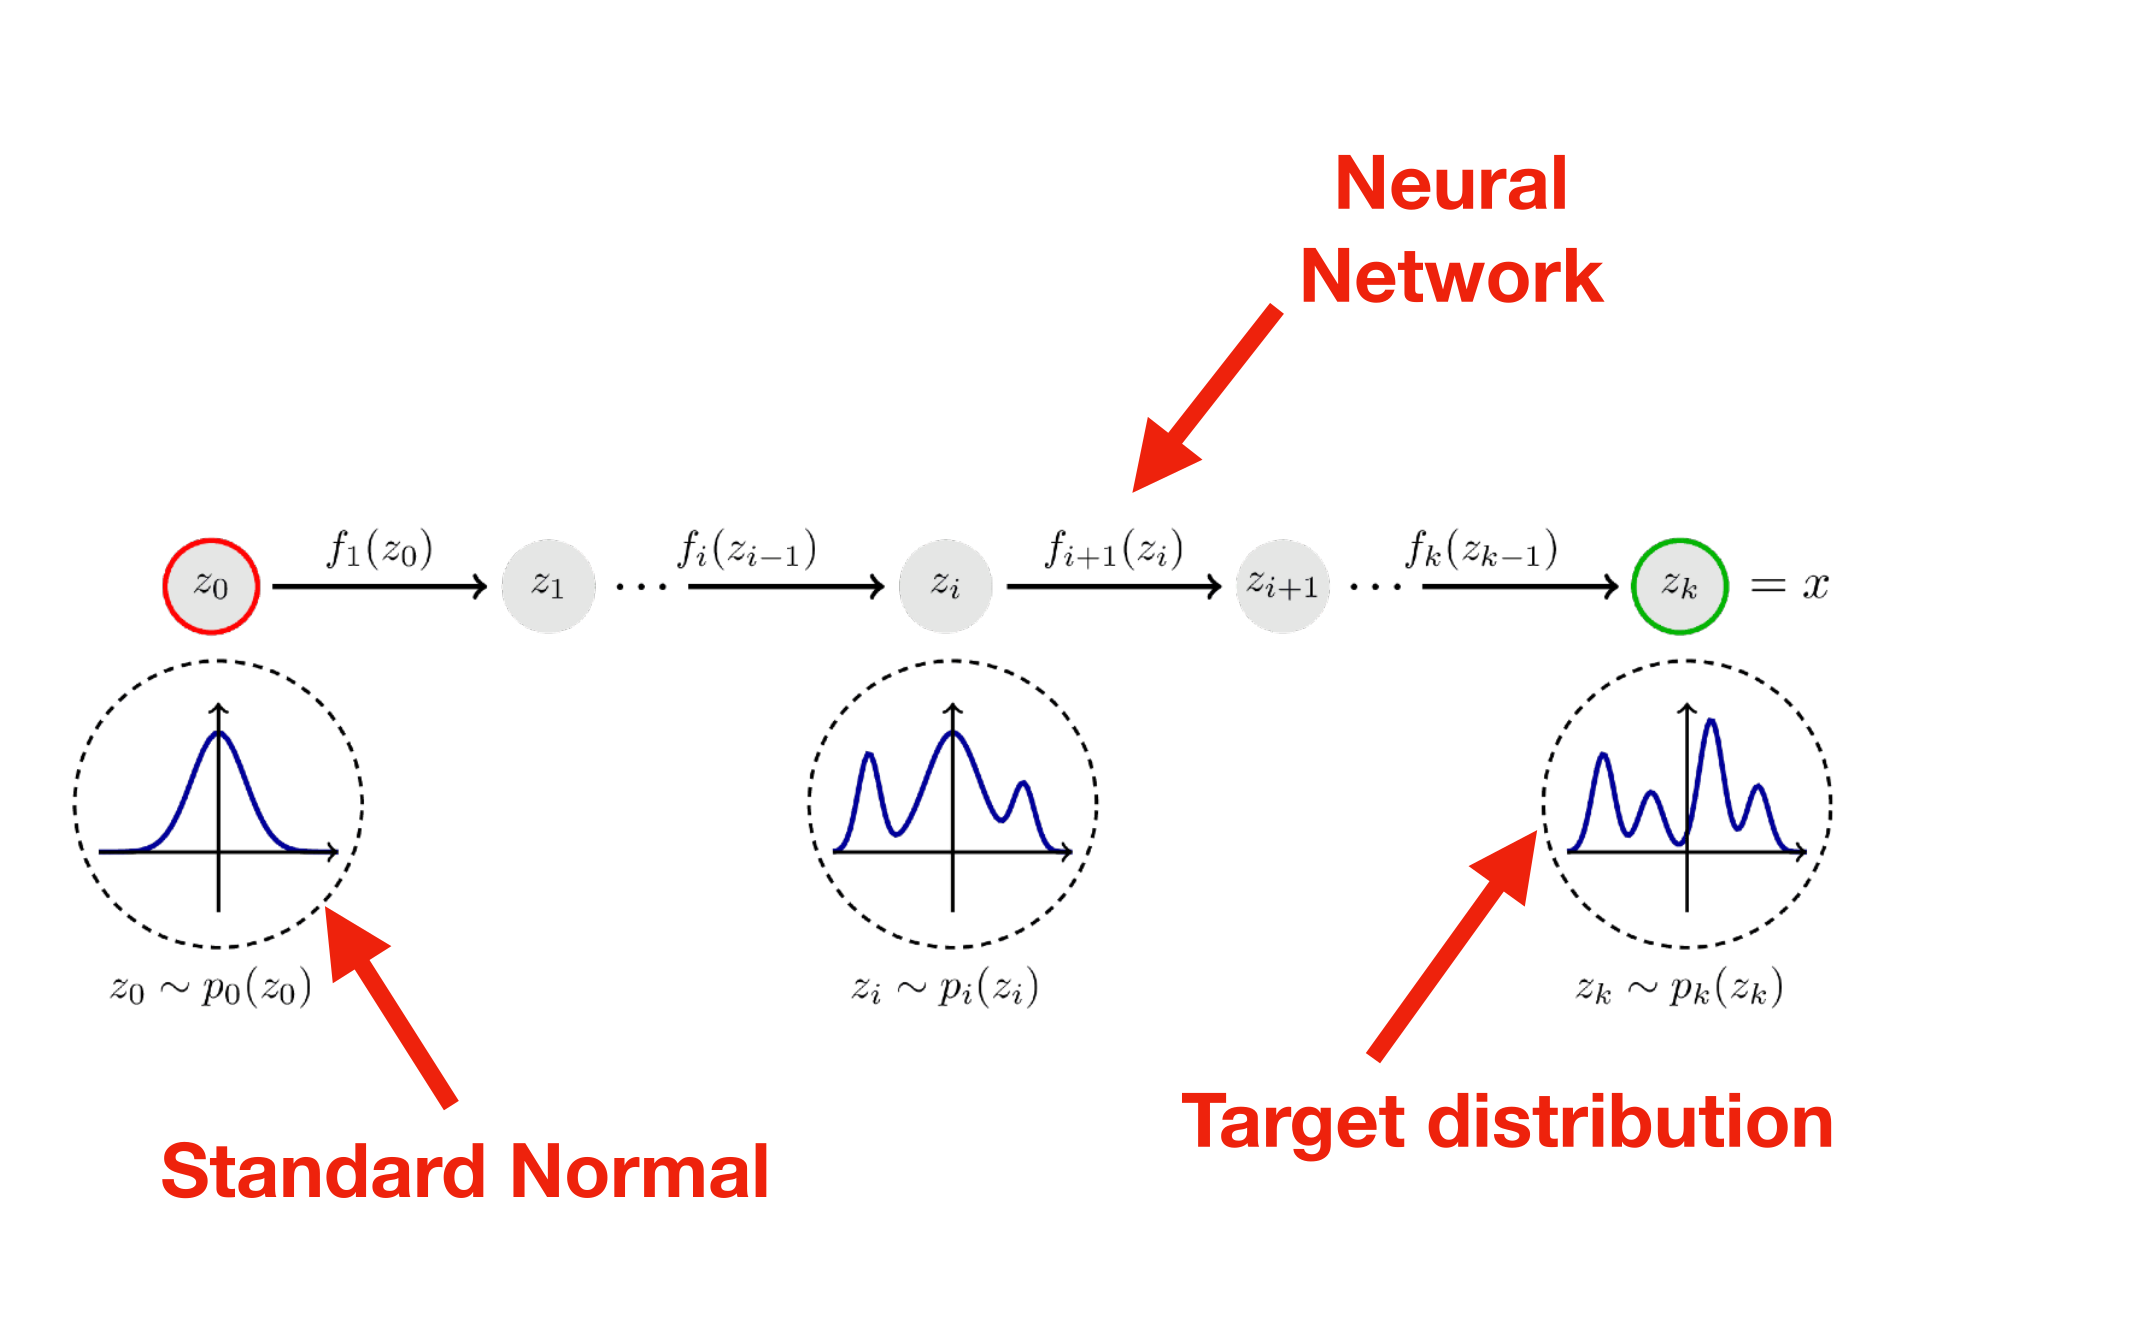
\includegraphics[width=0.5\textwidth]{Ca_Foscari Beamer/NF_diagram.png}}
\end{frame}

\begin{frame}{NF + PR}
\begin{itemize}\vspace{1em}
    \item<1-> Use \textbf{normalizing flows} (NF) to learn the rough \textcolor{RoyalBlue}{posterior}, and use this as our updated prior, $\pi^\ast$.
    \item<1-> In this case, can't do our trick of correcting the second \textcolor{red}{evidence} by volume ratio, $\frac{V_{\pi^\ast}}{V_{\pi}}$!
    \item<1-> Must rely on another technique to get around this!
\end{itemize}\vspace{2em}
\visible<2->{\textcolor{red}{Posterior repartitioning} (PR) can help us with this! (see e.g. \textcolor{cfgrey}{2212.01760})}\hspace{2em}\vfill
\begin{minipage}{1\textwidth}
\visible<2->{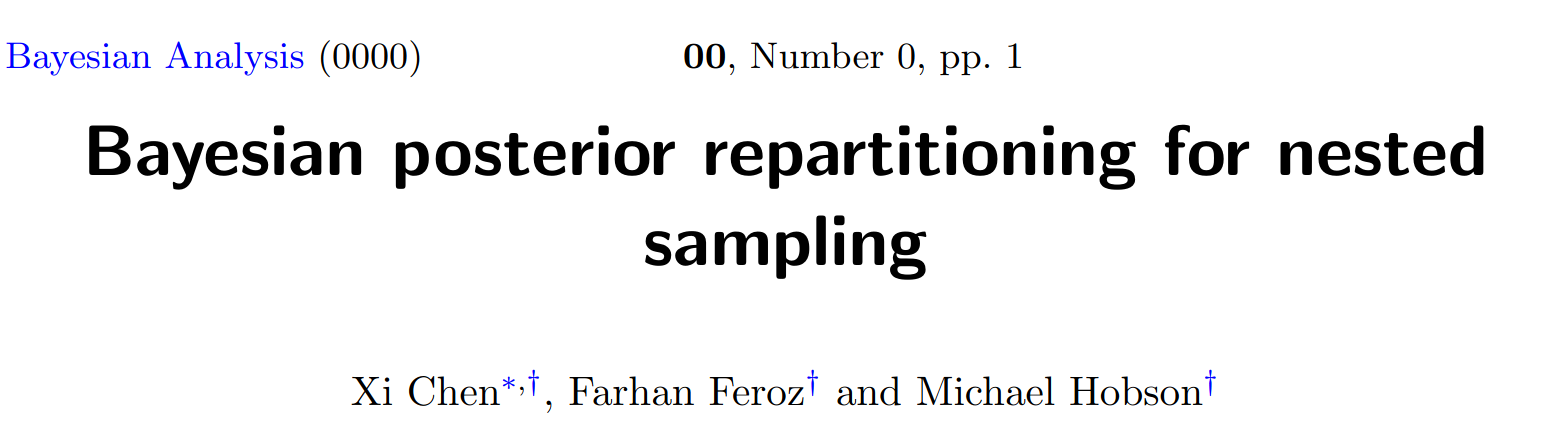
\includegraphics[width=0.3\textwidth]{Ca_Foscari Beamer/PR1.png}
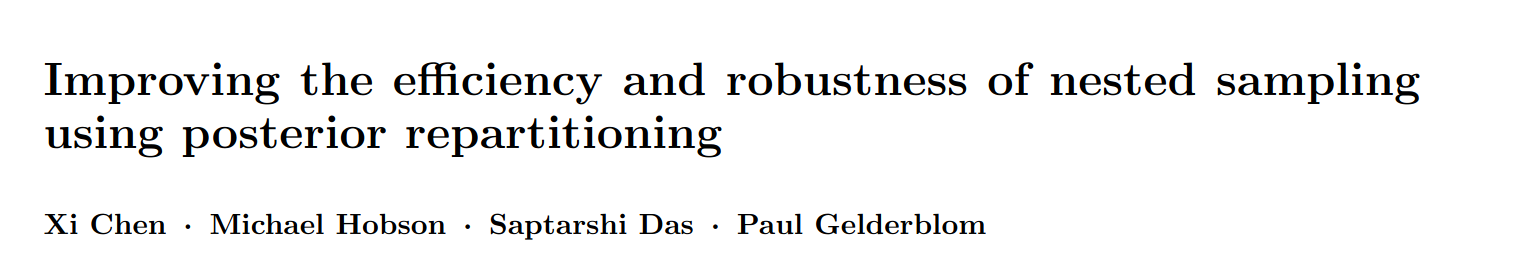
\includegraphics[width=0.38\textwidth]{Ca_Foscari Beamer/PR2.png}
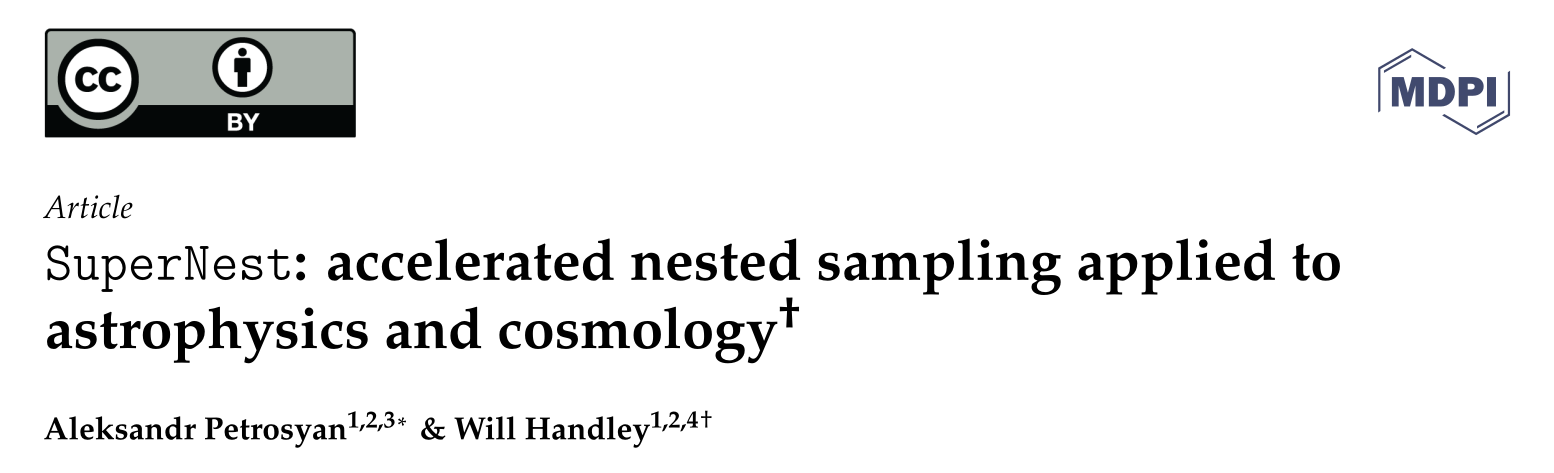
\includegraphics[width=0.3\textwidth]{Ca_Foscari Beamer/PR3.png}
}
\end{minipage}
\end{frame}

\begin{frame}{Posterior repartitioning (PR)}\vfill
\begin{itemize}
    \item \textcolor{red}{Evidence} and \textcolor{RoyalBlue}{posterior} only depend on product of $\mathcal{L}$ and $\pi$: \vspace{-2em}
\begin{multicols}{2}
\begin{equation}
    \textcolor{red}{\mathcal{Z}} = \int \textcolor{Purple}{\mathcal{L}(\theta)} \textcolor{BurntOrange}{\pi(\theta)} d\theta
\end{equation}\break
\begin{equation}
    \textcolor{RoyalBlue}{\mathcal{P}(\theta)} = \frac{\textcolor{Purple}{\mathcal{L}(\theta)} \textcolor{BurntOrange}{\pi(\theta)}}{\textcolor{red}{\mathcal{Z}}}
\end{equation}
\end{multicols}

    \bblock{We are free to redefine the likelihood and prior however we like - as long as the product is the same! \textcolor{cfgrey}{arXiv:1908.04655}}
    \centering
    \begin{equation}
        \textcolor{red}{\tilde{\mathcal{Z}}} = \int \textcolor{Purple}{\tilde{\mathcal{L}}(\theta)} \textcolor{BurntOrange}{\tilde{\pi}(\theta)} d\theta = \int \textcolor{Purple}{\mathcal{L}(\theta)} \textcolor{BurntOrange}{\pi(\theta)} d\theta = \textcolor{red}{\mathcal{Z}}
    \end{equation}
\eblock
\end{itemize}

\end{frame}

\begin{frame}{PR (cont.)}
\begin{itemize}

\vfill
     \item Many sampling algorithms do not distinguish between $\textcolor{Purple}{\mathcal{L}}$ and $\textcolor{BurntOrange}{\pi}$ at the algorithmic level.
    \item e.g. Metropolis-Hastings acceptance ratio only depends on the \textbf{joint distribution}, $\textcolor{Purple}{\mathcal{L}(\theta)} \textcolor{BurntOrange}{\pi(\theta)}$.
   \item Nested sampling does distinguish between prior and likelihood at the algorithmic level, by \textcolor{red}{`sampling from the prior $\pi$, subject to the hard likelihood constraint, $\mathcal{L}$'}.
\vfill
\item $\textcolor{red}{\mathcal{Z}}$ and $\textcolor{RoyalBlue}{\mathcal{P}}$ will not change if we repartition \textcolor{Purple}{$\mathcal{L}$} and \textcolor{BurntOrange}{$\pi$}, \textbf{but} $\boldsymbol{\mathcal{D}}_\mathbf{\mathrm{\textbf{KL}}}$ \textbf{will}.
\end{itemize}
\end{frame}

\begin{frame}{PR-NS w/ NFs}
    \centering
    \visible<1->{$\textcolor{BurntOrange}{\pi(\theta)} \longrightarrow \textcolor{BurntOrange}{\text{NF}(\theta)}$ }
    \vfill
    \visible<2->{$\textcolor{Purple}{\mathcal{L}(\theta)} \longrightarrow \textcolor{Purple}{\frac{\mathcal{L}(\theta)\pi(\theta)}{\text{NF}(\theta)}}$}
    \vfill
    \visible<3->{$\mathcal{D}_\mathrm{KL} \approx \text{log}\frac{V_\text{NF}}{V_\mathcal{P}}$}
\end{frame}

\begin{frame}{Demo on simulated example}
\begin{minipage}{0.45\textwidth}\vspace{1em}
\begin{itemize}
    \item<1-> Perform low resolution run on simulated data.
    \item<2-> Train NF on the weighted samples.
    \item<3-> Use this as `repartitioned prior' for new high resolution run (using PR to also update likelihood accordingly to same evidences and posteriors out).
\end{itemize}
\end{minipage}
\begin{minipage}{0.45\textwidth}
        \visible<1>{\vspace{2.5em}\begin{figure}
        \centering
        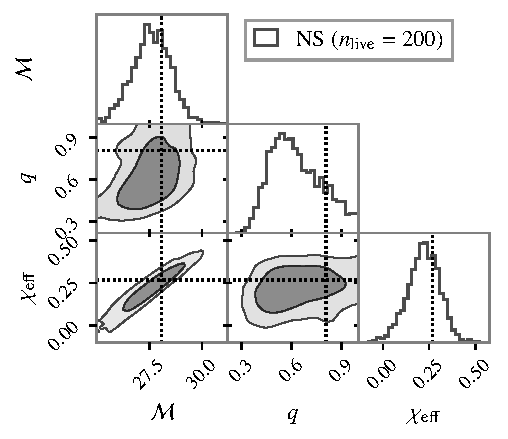
\includegraphics[]{Ca_Foscari Beamer/presentation_simulated_1.pdf}
    \end{figure}}
    \visible<2-3>{\vspace{-18.5em}\begin{figure}
        \centering
        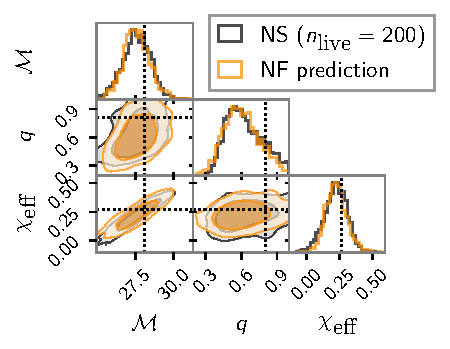
\includegraphics[]{Ca_Foscari Beamer/presentation_simulated_2.pdf}
    \end{figure}}
    \visible<4>{\vspace{-18em}\begin{figure}
        \centering
        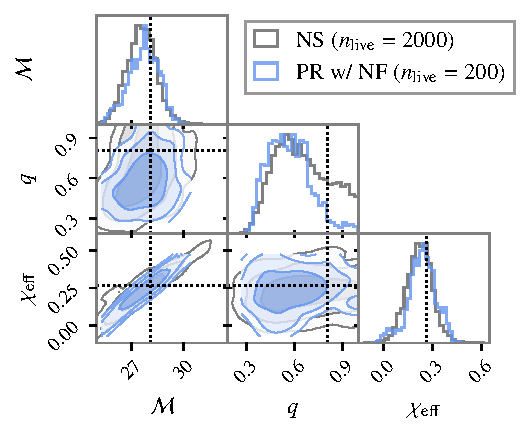
\includegraphics[]{Ca_Foscari Beamer/presentation_simulated_3.pdf}
    \end{figure}}
    \visible<5>{\vspace{-19em}\begin{figure}
        \centering
        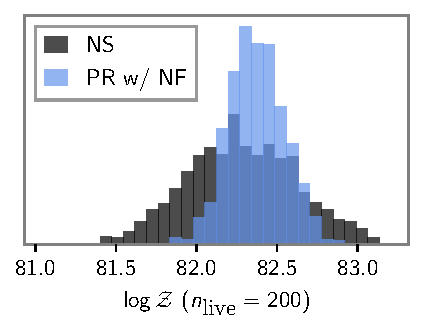
\includegraphics[]{Ca_Foscari Beamer/presentation_logZ_simulated.pdf}
    \end{figure}}
\end{minipage}

\vfill
\visible<5>{Same answer as doing a full resolution pass of NS, but \alert{7x faster} (precision-normalized)}.

\end{frame}

\begin{frame}{Potential pitfalls}

    \begin{itemize}
        \item If NF learns something \textbf{narrower} than true posterior, we can make the problem harder!
    \end{itemize}
    \begin{figure}
        \centering
        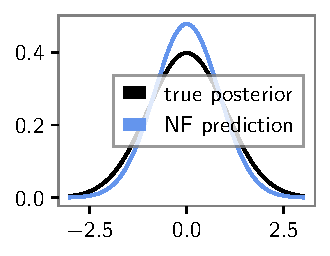
\includegraphics[]{Ca_Foscari Beamer/presentation_narrower_posterior.pdf}
    \end{figure}\vspace{-2em}
\end{frame}

\begin{frame}{Potential pitfalls (cont.)}
\vspace{2em}
    \begin{itemize}
    \item Still have an issue with multi-modality (if NF only learns one mode, the others are cut off at the prior level in the high resolution run).
\end{itemize}

    \begin{figure}
        \centering
        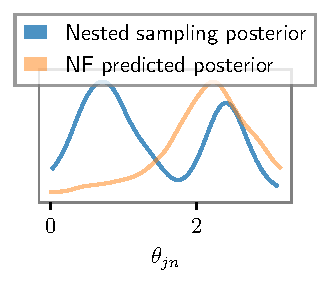
\includegraphics[]{Ca_Foscari Beamer/presentation_multimodality.pdf}
    \end{figure}
\end{frame}

\begin{frame}{Real GW example}
    When the NF has been unable to properly learn the multi-modality, we can get biased posteriors and evidences (GW191222):
 
    \begin{columns}

\column{0.5\textwidth}
\begin{figure}
    \centering
    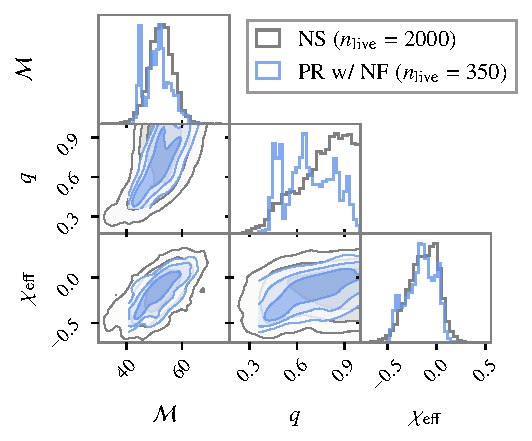
\includegraphics[width=0.75\linewidth]{Ca_Foscari Beamer/presentation_GW191222_1.pdf}
\end{figure}

\column{0.5\textwidth}
\begin{figure}
    \centering
    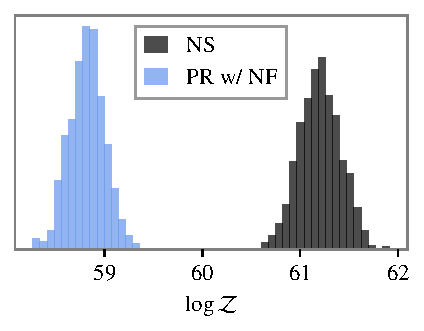
\includegraphics[width=0.75\linewidth]{Ca_Foscari Beamer/presentation_logZ_GW191222.pdf}
\end{figure}
\end{columns}
    
\end{frame}

\begin{frame}{Improving the method}
    In order to improve the robustness of the method: \vfill
    \begin{itemize}
        \item Repartitioned prior should ideally be able to \textbf{widen itself adaptively at runtime} to mitigate missed modes and badly learned posteriors.
    \end{itemize}
\end{frame}

%-----------------------------------------------------------------
\section{$\beta$-flows}

\begin{frame}{$\beta$-flows vs typical NFs}
    \begin{columns}
        \column{0.5\textwidth}\vspace{-40em}
        \begin{tikzpicture}
        \def\svgwidth{\textwidth}
        \hspace{-0em}
        \input{NS_cartoon_5.pdf_tex}
        \end{tikzpicture}
    \column{0.5\textwidth}
    \begin{itemize}
        \item Nested sampling sees tip to tail of the posterior in a systematic way, and NS has deep tails.
        \item NS can be used to train a specialized form of \textbf{conditional NFs} that can better learn these deep tail events.
        \item $\beta$-flows are new and only used in this work so far, though broadly applicable.
    \end{itemize}
    \end{columns}
\end{frame}

\begin{frame}{Better at deep tail probabilities}
    \begin{columns}
        \column{0.5\textwidth}\vspace{3em}
        \begin{figure}
            \centering
            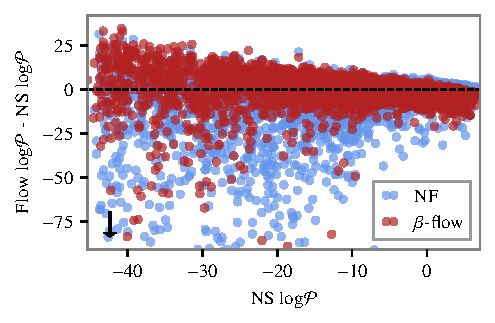
\includegraphics[width=0.9\textwidth]{Ca_Foscari Beamer/NF_vs_betaflow_simulated_v2.pdf}
        \end{figure}
    \column{0.5\textwidth}
    \begin{itemize}
        \item For simulated example shown before, the $\beta$-flow is able to better predict the NS posterior probabilities.
        \item $\beta$-flows exhibit less scatter in the tails (low posterior probabilities) than the NFs.
    \end{itemize}
    \end{columns}
\end{frame}

\begin{frame}{What is $\beta$?}
\begin{itemize}\vspace{2em}
    \item NS compresses step by step from prior to posterior.
    \item We can label these stages by a parameter $\beta$ (akin to inverse temperature $\beta$ in e.g. materials science). 
    \item Sliding scale from $\beta = 0$ as the prior and $\beta = 1$ as the posterior. 
\end{itemize}
\begin{figure}
    \centering
    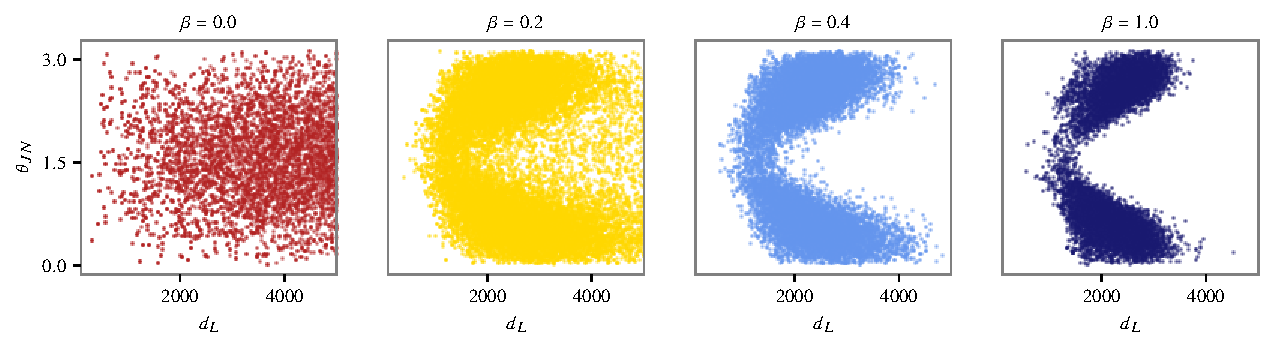
\includegraphics[width=0.9\textwidth]{Ca_Foscari Beamer/presentation_beta_extrinsic.pdf}
\end{figure}

\end{frame}

\begin{frame}{$\beta$-flows as adaptive prior}
\begin{columns}
\column{0.6\textwidth}
    \begin{itemize}
        \item We \textbf{sample over $\beta$} at runtime
        \item We can set the repartitioned prior to be anywhere between the posterior ($\beta=1$) and the original prior ($\beta=0$).
        \item Can \textbf{widen themselves adaptively} at runtime
    \end{itemize}\vspace{2em}
    \begin{equation}
        p(\beta) \propto \mathcal{L}^\beta \pi, \hspace{2em} \beta \in [0,1]
    \end{equation}
\column{0.34\textwidth}
\begin{figure}
    \centering
    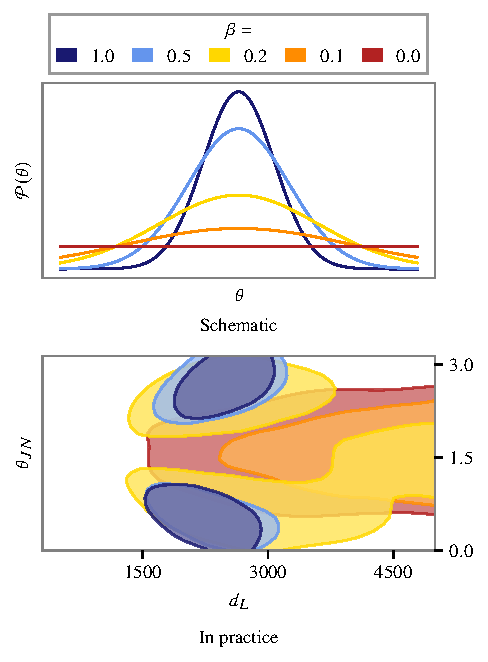
\includegraphics[width=1\textwidth]{Ca_Foscari Beamer/figure3_beta_v2.pdf}
\end{figure}
\end{columns}   
\end{frame}

%---------------------------------------------------------
%Highlighting text
\begin{frame}
\frametitle{GW191222 (again)}
    \begin{itemize}\vspace{2em}
        \item Using $\beta$-flows to set the repartitioned prior for the high resolution run, instead of a typical NF, and sampling over $\beta$ now fixes the problem.
    \end{itemize}
\begin{columns}
    \column{0.3\textwidth}
        \centering
        \includegraphics<2>[width=\linewidth]{Ca_Foscari Beamer/presentation_GW191222_1.pdf}%
        \includegraphics<3->[width=\linewidth]{Ca_Foscari Beamer/presentation_GW191222_1_beta.pdf}%
    \column{0.3\textwidth}
        \centering
        \includegraphics<2>[width=\linewidth]{Ca_Foscari Beamer/presentation_GW191222_2.pdf}%
        \includegraphics<3->[width=\linewidth]{Ca_Foscari Beamer/presentation_GW191222_2_beta.pdf}%
    \column{0.3\textwidth}
        \centering
        \includegraphics<2>[width=\linewidth]{Ca_Foscari Beamer/presentation_logZ_GW191222.pdf}%
        \includegraphics<3->[width=\linewidth]{Ca_Foscari Beamer/presentation_logZ_GW191222_beta.pdf}%
\end{columns}

\visible<4>{Only \textcolor{red}{2x} (precision-normalized) as fast as normal NS for this real example, but robust.}
\end{frame}
%---------------------------------------------------------

\begin{frame}{Summary}
    \begin{itemize}
        \item<1-> Several ways to reduce NS runtime, including reducing amount of compression from prior to posterior.
        \begin{itemize}
        \item<1-> Can perform low resolution run to identify rough posterior, learn distribution with a flow, and perform high resolution run with updated prior.
        \item<1-> Use posterior repartitioning to get correct \textcolor{red}{evidences} out, despite changed prior.
        \item<1-> Can achieve order of magnitude speedups on realistic GW examples.
        \end{itemize}\vfill
        \item<2-> Introduced $\beta$-flows:
        \begin{itemize}
            \item<2-> Conditional normalizing flow, trained with whole NS run
            \item<2-> Better at deep tail events
            \item<2-> First application is in this paper, but their use is much broader!
        \end{itemize}
    \end{itemize}
\end{frame}

\begin{frame}{}
    \centering
    Thank you for listening!
\end{frame}

% \begin{frame}{Posterior repartitioning (PR)}
% Unlike other sampling algorithms, such as Metropolis-Hastings or Hamiltonian Monte Carlo, NS distinguishes between $\mathcal{L}$ and $\pi$ by \alert{`sampling from the prior, subject to the hard likelihood constraint, $\mathcal{L}$'}.

% But evidence and posteriors only depend on product of $\mathcal{L}$ and $\pi$: \vspace{-2em}
% \begin{multicols}{2}
% \begin{equation}
%     \mathcal{Z} = \int \mathcal{L}(\theta) \pi(\theta) d\theta
% \end{equation}\break
% \begin{equation}
%     \mathcal{P}(\theta) = \frac{\mathcal{L}(\theta)\pi(\theta)}{\mathcal{Z}}
% \end{equation}
% \end{multicols}
% \bblock{Therefore, we are free to redefine the likelihood and prior however we like - as long as the product is the same! \textcolor{cfgrey}{arXiv:1908.04655}}
%     \centering
%     \begin{equation}
%         \tilde{\mathcal{Z}} = \int \tilde{\mathcal{L}}(\theta) \tilde{\pi}(\theta) d\theta = \int \mathcal{L}(\theta) \pi(\theta) d\theta = \mathcal{Z}
%     \end{equation}
% \eblock
% \end{frame}
% %---------------------------------------------------------

% %---------------------------------------------------------


% \begin{frame}{What is $\beta$?}
% \begin{itemize}\vspace{2em}
%     \item NS compresses step by step from prior to posterior.
%     \item We can label these stages by a parameter $\beta$ (akin to inverse temperature $\beta$ in e.g. materials science). 
%     \item Sliding scale from $\beta = 0$ as the prior and $\beta = 1$ as the posterior.
% \end{itemize}
% \begin{figure}
%     \centering
%     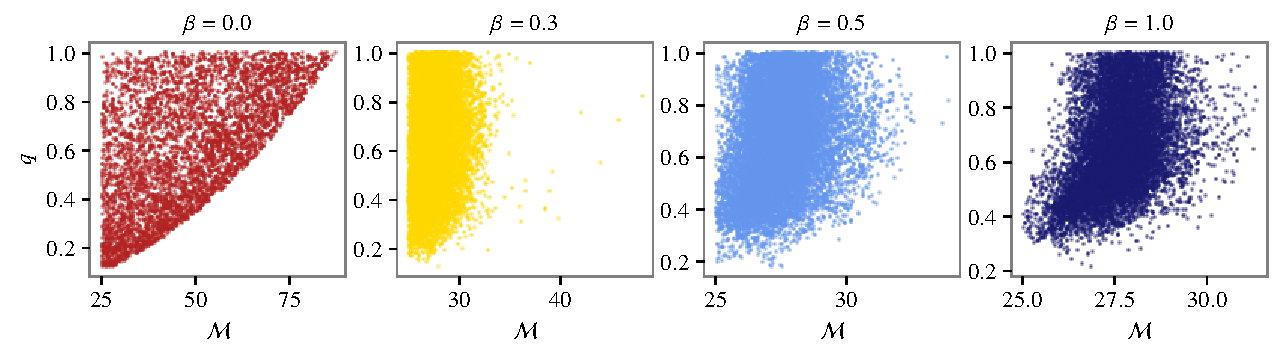
\includegraphics[width=0.9\linewidth]{Ca_Foscari Beamer/presentation_beta.pdf}
% \end{figure}

% \end{frame}

% \begin{frame}{Adaptive proposal}
% \begin{columns}
% \column{0.7\textwidth}
%     \begin{itemize}
%         \item $\beta$-flow can predict the ($\beta = 1$) posterior, similarly to NF (but better in tails).
%         \item Can predict \textbf{any intermediate stage} of NS too.
%         \item We \textbf{sample over $\beta$} at runtime, so proposal can now widen itself adaptively if modes have been missed!
%     \end{itemize}
% \column{0.3\textwidth}
% \begin{figure}
%     \centering
%     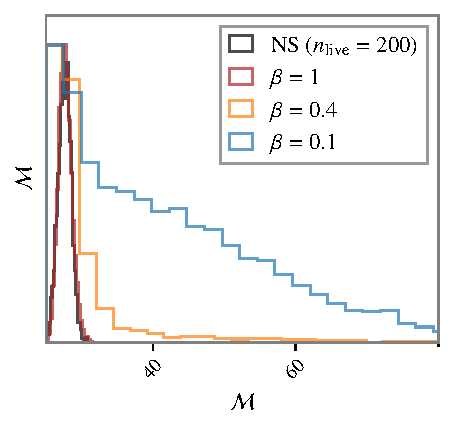
\includegraphics[width=1\textwidth]{Ca_Foscari Beamer/presentation_beta_1.pdf}
% \end{figure}
% \end{columns}   
% \end{frame}

\end{document}